%%%%%%%%%%%%%%%%%%%%%%%%%%%%%%%%%%%%%%%%%
% Lachaise Assignment
% LaTeX Template
% Version 1.0 (26/6/2018)
%
% This template originates from:
% http://www.LaTeXTemplates.com
%
% Authors:
% Marion Lachaise & François Févotte
% Vel (vel@LaTeXTemplates.com)
%
% License:
% CC BY-NC-SA 3.0 (http://creativecommons.org/licenses/by-nc-sa/3.0/)
% 
%%%%%%%%%%%%%%%%%%%%%%%%%%%%%%%%%%%%%%%%%

%----------------------------------------------------------------------------------------
%	PACKAGES AND OTHER DOCUMENT CONFIGURATIONS
%----------------------------------------------------------------------------------------
\documentclass{ctexart}
\usepackage{ctex}
\usepackage{graphicx}
\usepackage{float}
\usepackage{subfigure}
\usepackage{rotating}
\usepackage[svgnames]{xcolor} % Required for colour specification


\newcommand*{\plogo}{\fbox{$\mathcal{PL}$}} % Generic dummy publisher logo

\usepackage[utf8]{inputenc} % Required for inputting international characters
\usepackage[T1]{fontenc} % Output font encoding for international characters
\usepackage{PTSerif} % Use the Paratype Serif font

%\documentclass{article}

%%%%%%%%%%%%%%%%%%%%%%%%%%%%%%%%%%%%%%%%%
% Lachaise Assignment
% Structure Specification File
% Version 1.0 (26/6/2018)
%
% This template originates from:
% http://www.LaTeXTemplates.com
%
% Authors:
% Marion Lachaise & François Févotte
% Vel (vel@LaTeXTemplates.com)
%
% License:
% CC BY-NC-SA 3.0 (http://creativecommons.org/licenses/by-nc-sa/3.0/)
% 
%%%%%%%%%%%%%%%%%%%%%%%%%%%%%%%%%%%%%%%%%

%----------------------------------------------------------------------------------------
%	PACKAGES AND OTHER DOCUMENT CONFIGURATIONS
%----------------------------------------------------------------------------------------

\usepackage{amsmath,amsfonts,stmaryrd,amssymb} % Math packages

\usepackage{enumerate} % Custom item numbers for enumerations

\usepackage[ruled]{algorithm2e} % Algorithms

\usepackage[framemethod=tikz]{mdframed} % Allows defining custom boxed/framed environments

\usepackage{listings} % File listings, with syntax highlighting
\lstset{
	basicstyle=\ttfamily, % Typeset listings in monospace font
}

%----------------------------------------------------------------------------------------
%	DOCUMENT MARGINS
%----------------------------------------------------------------------------------------

\usepackage{geometry} % Required for adjusting page dimensions and margins

\geometry{
	paper=a4paper, % Paper size, change to letterpaper for US letter size
	top=2.5cm, % Top margin
	bottom=3cm, % Bottom margin
	left=2.5cm, % Left margin
	right=2.5cm, % Right margin
	headheight=14pt, % Header height
	footskip=1.5cm, % Space from the bottom margin to the baseline of the footer
	headsep=1.2cm, % Space from the top margin to the baseline of the header
	%showframe, % Uncomment to show how the type block is set on the page
}

%----------------------------------------------------------------------------------------
%	FONTS
%----------------------------------------------------------------------------------------

\usepackage[utf8]{inputenc} % Required for inputting international characters
\usepackage[T1]{fontenc} % Output font encoding for international characters

\usepackage{XCharter} % Use the XCharter fonts

%----------------------------------------------------------------------------------------
%	COMMAND LINE ENVIRONMENT
%----------------------------------------------------------------------------------------

% Usage:
% \begin{commandline}
%	\begin{verbatim}
%		$ ls
%		
%		Applications	Desktop	...
%	\end{verbatim}
% \end{commandline}

\mdfdefinestyle{commandline}{
	leftmargin=10pt,
	rightmargin=10pt,
	innerleftmargin=15pt,
	middlelinecolor=black!50!white,
	middlelinewidth=2pt,
	frametitlerule=false,
	backgroundcolor=black!5!white,
	frametitle={Command Line},
	frametitlefont={\normalfont\sffamily\color{white}\hspace{-1em}},
	frametitlebackgroundcolor=black!50!white,
	nobreak,
}

% Define a custom environment for command-line snapshots
\newenvironment{commandline}{
	\medskip
	\begin{mdframed}[style=commandline]
}{
	\end{mdframed}
	\medskip
}

%----------------------------------------------------------------------------------------
%	FILE CONTENTS ENVIRONMENT
%----------------------------------------------------------------------------------------

% Usage:
% \begin{file}[optional filename, defaults to "File"]
%	File contents, for example, with a listings environment
% \end{file}

\mdfdefinestyle{file}{
	innertopmargin=1.6\baselineskip,
	innerbottommargin=0.8\baselineskip,
	topline=false, bottomline=false,
	leftline=false, rightline=false,
	leftmargin=2cm,
	rightmargin=2cm,
	singleextra={%
		\draw[fill=black!10!white](P)++(0,-1.2em)rectangle(P-|O);
		\node[anchor=north west]
		at(P-|O){\ttfamily\mdfilename};
		%
		\def\l{3em}
		\draw(O-|P)++(-\l,0)--++(\l,\l)--(P)--(P-|O)--(O)--cycle;
		\draw(O-|P)++(-\l,0)--++(0,\l)--++(\l,0);
	},
	nobreak,
}

% Define a custom environment for file contents
\newenvironment{file}[1][File]{ % Set the default filename to "File"
	\medskip
	\newcommand{\mdfilename}{#1}
	\begin{mdframed}[style=file]
}{
	\end{mdframed}
	\medskip
}

%----------------------------------------------------------------------------------------
%	NUMBERED QUESTIONS ENVIRONMENT
%----------------------------------------------------------------------------------------

% Usage:
% \begin{question}[optional title]
%	Question contents
% \end{question}

\mdfdefinestyle{question}{
	innertopmargin=1.2\baselineskip,
	innerbottommargin=0.8\baselineskip,
	roundcorner=5pt,
	nobreak,
	singleextra={%
		\draw(P-|O)node[xshift=1em,anchor=west,fill=white,draw,rounded corners=5pt]{%
		Question \theQuestion\questionTitle};
	},
}

\newcounter{Question} % Stores the current question number that gets iterated with each new question

% Define a custom environment for numbered questions
\newenvironment{question}[1][\unskip]{
	\bigskip
	\stepcounter{Question}
	\newcommand{\questionTitle}{~#1}
	\begin{mdframed}[style=question]
}{
	\end{mdframed}
	\medskip
}

%----------------------------------------------------------------------------------------
%	WARNING TEXT ENVIRONMENT
%----------------------------------------------------------------------------------------

% Usage:
% \begin{warn}[optional title, defaults to "Warning:"]
%	Contents
% \end{warn}

\mdfdefinestyle{warning}{
	topline=false, bottomline=false,
	leftline=false, rightline=false,
	nobreak,
	singleextra={%
		\draw(P-|O)++(-0.5em,0)node(tmp1){};
		\draw(P-|O)++(0.5em,0)node(tmp2){};
		\fill[black,rotate around={45:(P-|O)}](tmp1)rectangle(tmp2);
		\node at(P-|O){\color{white}\scriptsize\bf !};
		\draw[very thick](P-|O)++(0,-1em)--(O);%--(O-|P);
	}
}

% Define a custom environment for warning text
\newenvironment{warn}[1][Warning:]{ % Set the default warning to "Warning:"
	\medskip
	\begin{mdframed}[style=warning]
		\noindent{\textbf{#1}}
}{
	\end{mdframed}
}

%----------------------------------------------------------------------------------------
%	INFORMATION ENVIRONMENT
%----------------------------------------------------------------------------------------

% Usage:
% \begin{info}[optional title, defaults to "Info:"]
% 	contents
% 	\end{info}

\mdfdefinestyle{info}{%
	topline=false, bottomline=false,
	leftline=false, rightline=false,
	nobreak,
	singleextra={%
		\fill[black](P-|O)circle[radius=0.4em];
		\node at(P-|O){\color{white}\scriptsize\bf i};
		\draw[very thick](P-|O)++(0,-0.8em)--(O);%--(O-|P);
	}
}

% Define a custom environment for information
\newenvironment{info}[1][Info:]{ % Set the default title to "Info:"
	\medskip
	\begin{mdframed}[style=info]
		\noindent{\textbf{#1}}
}{
	\end{mdframed}
}
 % Include the file specifying the document structure and custom commands

%----------------------------------------------------------------------------------------
%	ASSIGNMENT INFORMATION
%----------------------------------------------------------------------------------------

%\title{\textbf{2020年秋商务智能}\textit{\ \ 大作业}} % Title of the assignment

%\author{姓名:王帅\ \ \ \ \ 学号: 2018302412 \\ \texttt{wangshuai.excellent@foxmail.com}} % Author name and email address

%\date{西北工业大学 计算机学院 --- \today} % University, school and/or department name(s) and a date

%----------------------------------------------------------------------------------------

\begin{document}

%\maketitle % Print the title

%----------------------------------------------------------------------------------------
%	INTRODUCTION
%----------------------------------------------------------------------------------------

\begin{titlepage} % Suppresses headers and footers on the title page
	
	\centering % Centre all text
	
	%------------------------------------------------
	%	Title and subtitle
	%------------------------------------------------
	
	\setlength{\unitlength}{0.6\textwidth} % Set the width of the curly brackets above and below the titles
	
	{\color{LightGoldenrod}\resizebox*{\unitlength}{\baselineskip}{\rotatebox{90}{$\}$}}}\\[\baselineskip] % Top curly bracket
	
	\textcolor{Sienna}{\textit{\Huge 二零年秋\ 商务智能大作业}}\\[\baselineskip] % Title
	
	{\color{RosyBrown}\Large Regression Analysis }\\ % Subtitle or further description
	
	{\color{LightGoldenrod}\resizebox*{\unitlength}{\baselineskip}{\rotatebox{-90}{$\}$}}} % Bottom curly bracket
	
	\vfill % Whitespace between the title and the author name
	
	%------------------------------------------------
	%	Author
	%------------------------------------------------
\textcolor{black}{\textit{\Large 姓名: \ \ \ \ \ \ \        王帅\ \ \ \ \ \ }}\\[\baselineskip] % Title
\textcolor{black}{\textit{\Large 学号: 2018302412}}\\[\baselineskip] % Title
\textcolor{black}{\textit{ 邮箱: wangshuai.excellent@foxmail.com}}\\[\baselineskip] % Title
	\vfill % Whitespace between the author name and the publisher logo
	
	%------------------------------------------------
	%	Publisher
	%------------------------------------------------
	
	\plogo\\[0.5\baselineskip] % Publisher logo
	
	西北工业大学计算机学院 % Publisher name
	
\end{titlepage}

\tableofcontents
\section*{前言} % Unnumbered section

商务智能大作业要求实现关联规则发现,聚类分析,分类,回归,链路预测相关算法中的一种,基于自己对于回归分析的兴趣,我选择回归分析作为本次大作业的研究方向,探讨不同的回归算法对于同一问题的效果,实现回归可视化效果以及误差对比,包括线性回归,多项式回归,岭回归算法,以及最后的支持向量回归SVR。

% Math equation/formula
\begin{equation}
	Y = f(\vec{X}, \beta) + error
\end{equation}

回归分析算法可以简单描述为:\ 拥有观测数据$X_{i}$,以及目标数据$Y$,以及未知变量$\beta$,整个问题可以表达为上式,其中$f(\vec{X}, \beta)$根据各个算法不同有不同的形式

\begin{info} % Information block
	在本次实验中,部分问题下,我把每个变量看成是随机变量,在短时间内和时间无关,也就是他们不是随机过程,而只是一个简单的随机变量,这样有助于分析问题,后面部分会详细说明。
\end{info}


%----------------------------------------------------------------------------------------
%	PROBLEM 1
%----------------------------------------------------------------------------------------

\section{数据集介绍} % Numbered section

本次实验选择UCI数据集集合中的\ \ \ 大气质量检测数据,实现基于这些数据的回归分析

%------------------------------------------------

\subsection{数据集信息}
The dataset contains 9358 instances of hourly averaged responses from an array of 5 metal oxide chemical sensors embedded in an Air Quality Chemical Multisensor Device. The device was located on the field in a significantly polluted area, at road level,within an Italian city. Data were recorded from March 2004 to February 2005 (one year)representing the longest freely available recordings of on field deployed air quality chemical sensor devices responses. Ground Truth hourly averaged concentrations for CO, Non Metanic Hydrocarbons, Benzene, Total Nitrogen Oxides (NOx) and Nitrogen Dioxide (NO2) and were provided by a co-located reference certified analyzer. Evidences of cross-sensitivities as well as both concept and sensor drifts are present as described in De Vito et al., Sens. And Act. B, Vol. 129,2,2008 (citation required) eventually affecting sensors concentration estimation capabilities. Missing values are tagged with -200 value. 


\textbf{翻译}:该数据集包含来自空气质量化学多传感器设备中的5个金属氧化物化学传感器阵列每小时平均响应的9358个实例。该设备位于意大利城市内道路污染严重的地区的田野上。从2004年3月到2005年2月(一年)记录了数据,这些数据是现场部署的空气质量化学传感器设备响应的最长免费记录。一氧化碳,非代谢碳氢化合物,苯,总氮氧化物(NOx)和二氧化氮(NO2)的地面真实小时平均浓度由共同定位的参考认证分析仪提供。如De Vito等人在《 Sens。And Act》中所述,存在交叉敏感性以及概念漂移和传感器漂移的证据。 B卷129,2,2008(需要引用)最终影响传感器浓度估算能力。缺少的值用-200值标记。
% Numbered question, with subquestions in an enumerate environment
%\begin{question}
%	Quisque ullamcorper placerat ipsum. Cras nibh. Morbi vel justo vitae lacus tincidunt ultrices. Lorem ipsum dolor sit amet, consectetuer adipiscing elit.

	% Subquestions numbered with letters
%	\begin{enumerate}[(a)]
%		\item Do this.
%		\item Do that.
%		\item Do something else.
%	\end{enumerate}
%\end{question}
	
%------------------------------------------------

\subsection{数据集内容}
\begin{enumerate}[(a)]
	\item Date (DD/MM/YYYY)
	\item Time (HH.MM.SS)
	\item True hourly averaged concentration CO in $mg/m^3$ (reference analyzer)
	\item PT08.S1 (tin oxide) hourly averaged sensor response (nominally CO targeted)
	\item True hourly averaged overall Non Metanic HydroCarbons concentration in $microg/m^3$ (reference analyzer)
	\item True hourly averaged Benzene concentration in $microg/m^3$ (reference analyzer)
	\item  PT08.S2 (titania) hourly averaged sensor response (nominally NMHC targeted)
	\item True hourly averaged NOx concentration in ppb (reference analyzer)
	\item PT08.S3 (tungsten oxide) hourly averaged sensor response (nominally NOx targeted)
	\item True hourly averaged NO2 concentration in $microg/m^3$ (reference analyzer)
	\item PT08.S4 (tungsten oxide) hourly averaged sensor response (nominally NO2 targeted)
	\item PT08.S5 (indium oxide) hourly averaged sensor response (nominally O3 targeted)
	\item Temperature in $°C$
	\item Relative Humidity (\%)
	\item AH Absolute Humidity 
\end{enumerate}

\subsection{数据清洗与数据划分}
阅读相关介绍,我们知道,这部分数据有脏数据,这部分数据是由于传感器故障或者其他原因,都被简单的标注为$-200$,本实验的数据清洗正式将这部分有脏数据的数据条目去掉。同时将数据归为验证数据,其余为训练数据。
以及最重要的,我本次是对RH,也就是相对湿度进行回归预测,然后衡量误差范围。
\subparagraph{统计脏数据} 通过对数据的统计,我们能更加清楚的知道,数据清洗的策略,如果盲目的直接去掉包含-200的行则会造成大量的浪费,举例来说,NMHC丢失了几乎所有数据,应该将这些数据直接去掉 \\
\begin{table}
	\centering
	\begin{tabular}{|c|c|}
		\hline
		数据 & 丢失数据数目 \\
		\hline
		CO(GT) & 1683 \\
		\hline
		PT08.S1(CO) & 366 \\
		\hline
		NMHC(GT) & 8443 \\
		\hline
		C6H6(GT) & 366 \\
		\hline
		PT08.S2(NMHC) & 366 \\
		\hline
		NOx(GT) & 1639 \\	
		\hline
		PT08.S3(NOx) & 366 \\
		\hline
		NO2(GT) & 1642 \\
		\hline
		PT08.S4(NO2) & 366 \\
		\hline
		PT08.S5(O3) & 366 \\
		\hline
		T & 366 \\
		\hline
		RH & 366 \\
		\hline
		AH & 366 \\
		\hline
	\end{tabular}
\end{table}
\begin{figure}[H]
	%\centering
	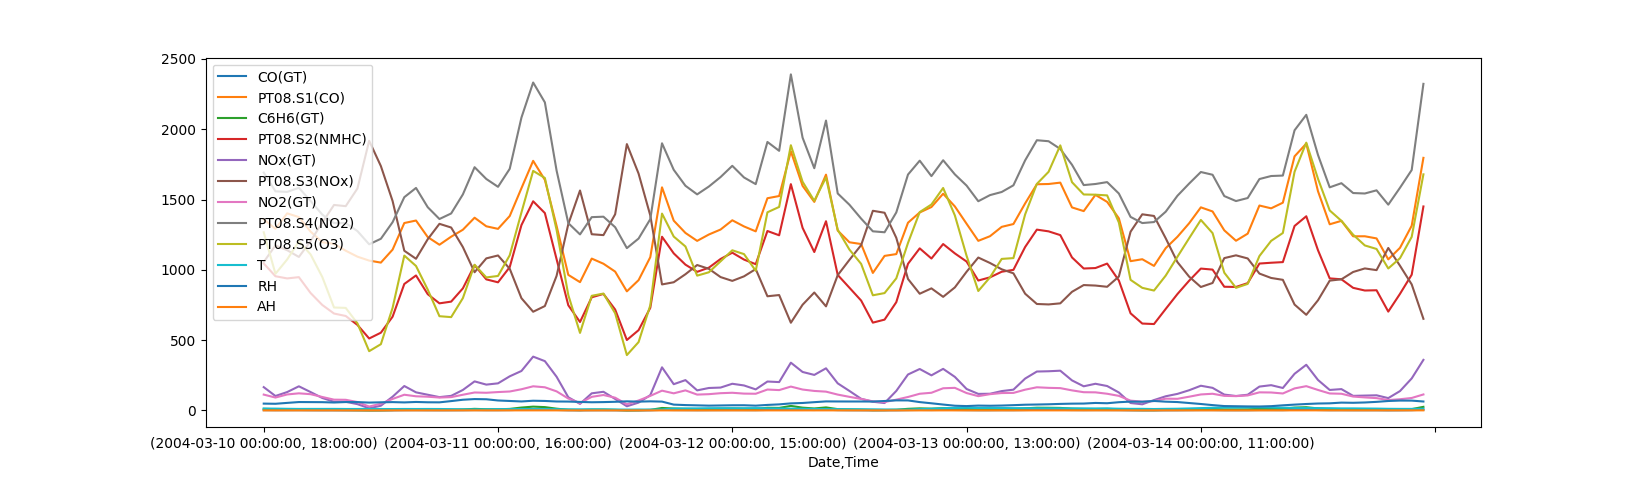
\includegraphics[width=1.2\textwidth]{../images/Figure_s.png}
	\caption{数据可视化}
\end{figure}
%\begin{sidewaystable}	
\begin{tabular}{|c|c|c|c|c|c|c|c|c|c|c|c|c}
\hline
属性&CO&S1&C6H6&NOx&S3&NO2&S4&S5&T&RH&AH \\
\hline
count&6941&6941&6941&6941&6941&6941&6941&6941&6941&6941&6941 \\
\hline
mean&2.18&1119&10.55&250.6&816.77&113.8&1452&1057&17.75&48.88&0.98\\
\hline
std&1.44&218.7&7.46&208.6&251.89&47.46&353.2&406.5&8.84&17.43&0.40\\
\hline
min&0.1&647.2&0.18&2.0&322.0&2.0&551.0&221.0&-1.8&9.19&0.184\\
\hline
25\%&1.1&956.2&4.98&103.0&642.2&79.0&1206&759.5&11.20&35.9&0.6922\\
\hline
50\%&1.9&1084&8.788&186.0&785.5&110.0&1457&1006&16.8&49.17&0.95\\
\hline
75\%&2.9&1254&14.57&334.6&946.5&142.0&1683&1322&23.29&62.22&1.25\\
\hline
max&11.9&2039&63.74&1479&2682&332.6&2775&2522&44.60&88.72&2.18\\
\hline
\end{tabular}

\begin{figure}[H]
	\centering
	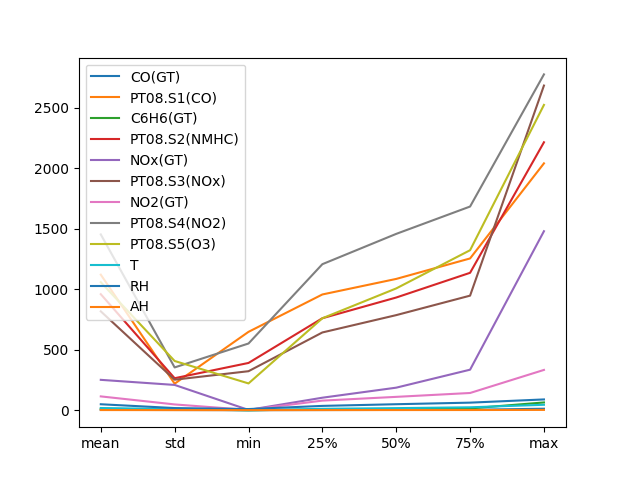
\includegraphics[width=0.8\textwidth]{../images/data.png}
	\caption{数据属性可视化}
\end{figure}

%\end{sidewaystable}
\subsection{数据相关程度分析}
\subparagraph{相关性矩阵可视化}
相关性矩阵是通过计算每个变量间的协方差,然后将协方差的值可视化出来,值越大代表两个变量之间的相关程度越高
\begin{figure}[H]
	\centering
	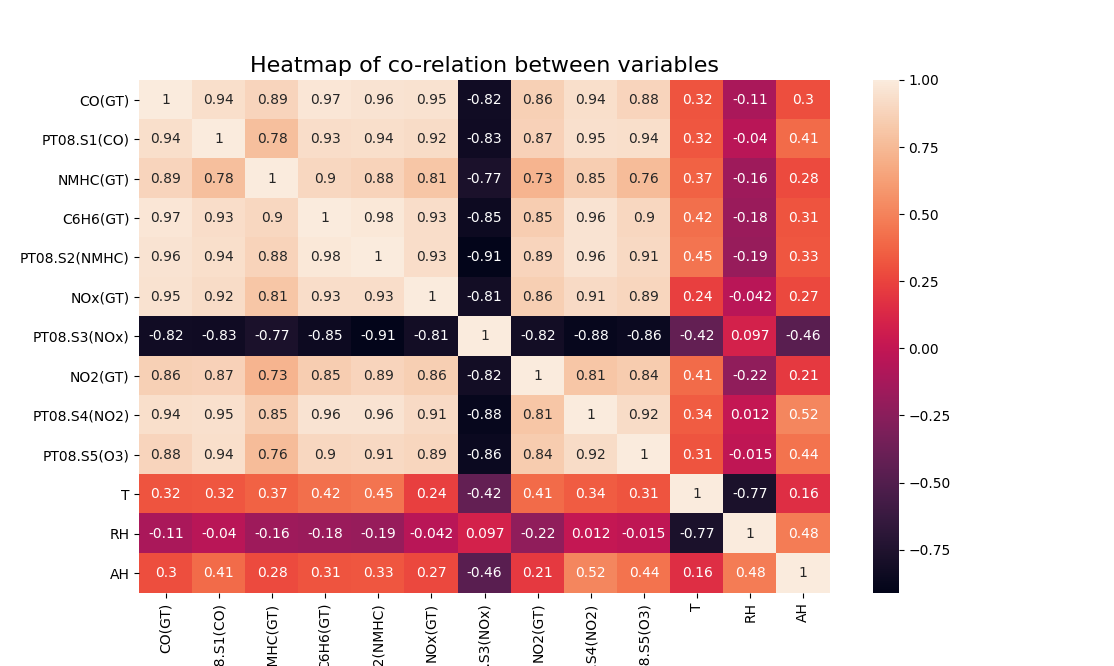
\includegraphics[width=1.3\textwidth]{../images/Figure_1.png}
	\caption{相关性矩阵}
\end{figure}
\section{线性回归}
\subsection{算法介绍}
线性回归是利用数理统计中回归分析,来确定两种或两种以上变量间相互依赖的定量关系的一种统计分析方法,运用十分广泛。其表达形式为$Y = W^T X + e$,e为误差服从均值为0的正态分布。回归分析中,只包括一个自变量和一个因变量,且二者的关系可用一条直线近似表示,这种回归分析称为一元线性回归分析。如果回归分析中包括两个或两个以上的自变量,且因变量和自变量之间是线性关系,则称为多元线性回归分析。一般来说,线性回归采用最小二乘法,通过回归来确定系数。 \\
一般地,影响y的因素往往不止一个,假设有$x_1,x_2,...,x_k$,$k$个因素,通常可考虑如下的线性关系式:
\begin{equation}
		y = \beta_0 + \beta_1 \ x_1 + \beta_2 \ x_2 + ... + \beta_k \ x_k + \epsilon
\end{equation}
对y与$x_1,x_2,...,x_k$同时作n次独立观察得n组观测值$(x_t1,x_t2,...,x_tk),t=1,2,...,n(n>k+1)$,它们满足关系式:
\begin{equation}
	y_t = \beta_0 + \beta_1 \ x_t1 + \beta_2 \ x_t2 + ... + \beta_k \ x_tk + \epsilon_t
\end{equation}
其中,$\epsilon_t$互不相关均是与$\epsilon$同分布的随机变量。用矩阵表示上式,可得:
\begin{equation}
Y =  \beta X + \epsilon 
\end{equation}
利用最小二乘法可以解得:
\begin{equation}
 \hat{\beta}  = (X^T \ X)^{-1} \ X^T \ Y  
\end{equation}
同时就本题来说,完全可以考虑加权,因为有些变量方差较大,变化过大,可以适当考虑赋予一个权重,其中权重和方差为反比,则可以有:
\begin{equation}
\hat{\beta}  = (X^T \ W X)^{-1} \ X^T \ W Y ................. (W = R^{-1})
\end{equation}

\subsection{算法实现}
\begin{info} % Information block
	这部分只贴了核心代码,第一个sigleX是单变量线性回归方案,第二个mutiX是多变量线性回归方案,
	采用python代码风格来表达算法流程。同时这里代码非常简短,就没有采用注释来说明细节。
\end{info}
\begin{file}[sigleX.py]
	\begin{lstlisting}[language=Python]
#! /usr/bin/python	
import numpy as np
def sigalX(X, Y):
  X = np.array(X)
  X = np.stack([X, np.ones(X.shape[0])], 1)
  print(X.shape)
  Y = np.array(Y)
  XTXinv=np.linalg.inv(np.matmul(X.transpose(),X))
  XTY = np.matmul(X.transpose(), Y)
  return np.matmul(XTXinv, XTY)
	\end{lstlisting}
\end{file}
\begin{file}[mutiX.py]
	\begin{lstlisting}[language=Python]
#! /usr/bin/python
def mutiX(X, Y):
  X = np.stack([*X, np.ones(X.shape[0])], 1)
  print(X.shape)
  Y = np.array(Y)
  XTXinv=np.linalg.inv(np.matmul(X.transpose(),X))
  XTY = np.matmul(X.transpose(), Y)
  return np.matmul(XTXinv, XTY)
	\end{lstlisting}
\end{file}
\subsection{单变量数据之间的线性性}
可以观察下面,线性性曲线,可以发现,温度,绝对湿度和相对湿度线性关系较为明显,下文选择这两个变量来研究问题。
\begin{figure}[H]
	\centering
	\subfigure{
	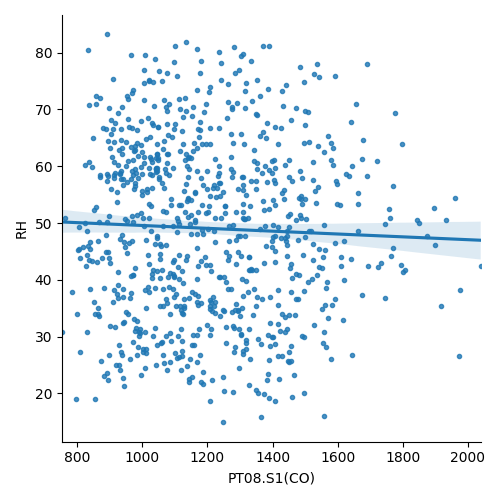
\includegraphics[width=0.3\textwidth]{../images/Figure_2.png}
	\label{线性性}
	}
	\subfigure{
		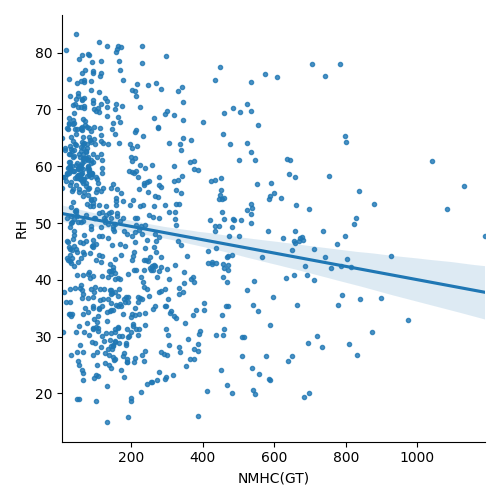
\includegraphics[width=0.3\textwidth]{../images/Figure_3.png}
		\label{线性性}
	}
		\subfigure{
		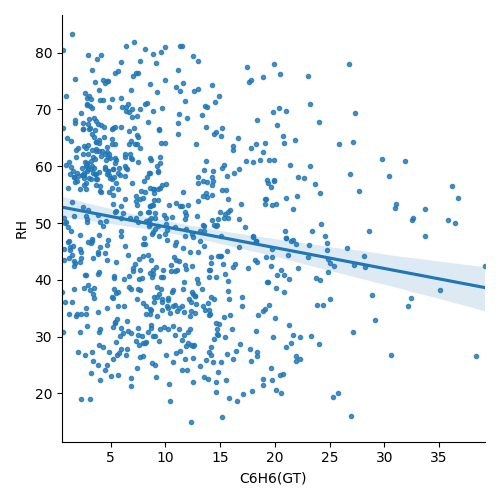
\includegraphics[width=0.3\textwidth]{../images/Figure_4.png}
		\label{线性性}
	}
	\subfigure{
	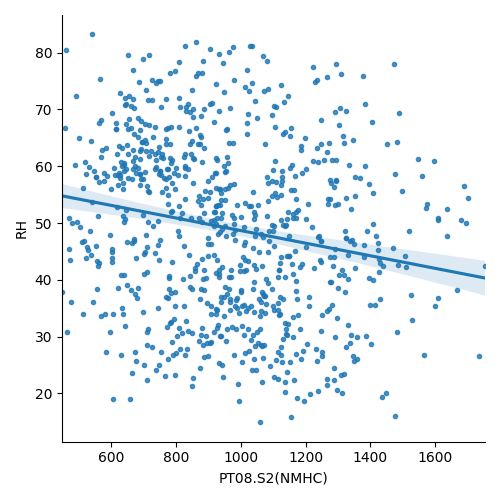
\includegraphics[width=0.3\textwidth]{../images/Figure_5.png}
	\label{线性性}
	}
	\subfigure{
	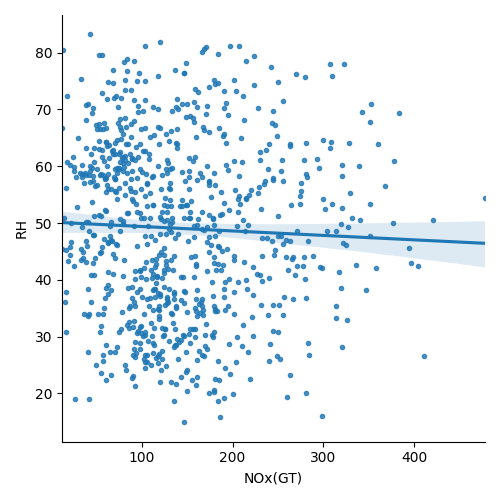
\includegraphics[width=0.3\textwidth]{../images/Figure_6.png}
	\label{线性性}
	}
	\subfigure{
	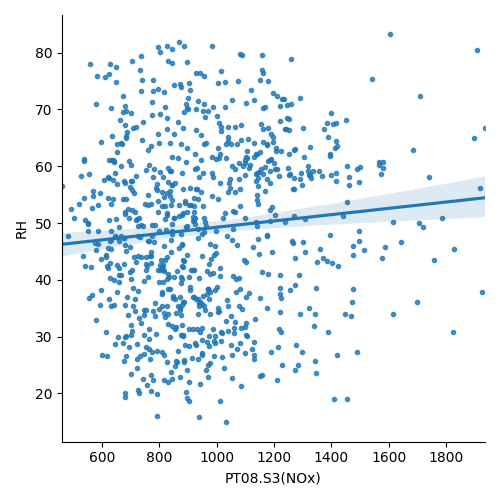
\includegraphics[width=0.3\textwidth]{../images/Figure_7.png}
	\label{线性性}
	}
	\subfigure{
	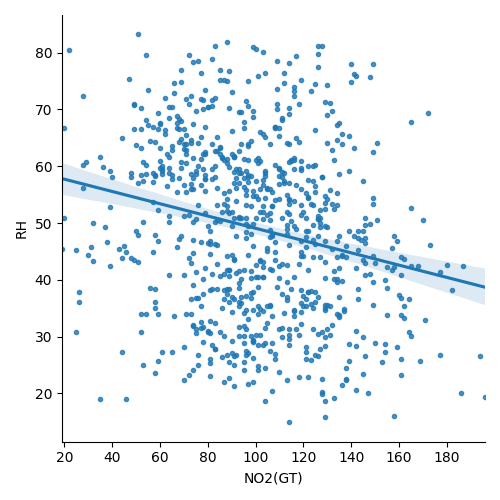
\includegraphics[width=0.3\textwidth]{../images/Figure_8.png}
	\label{线性性}
	}
	\subfigure{
	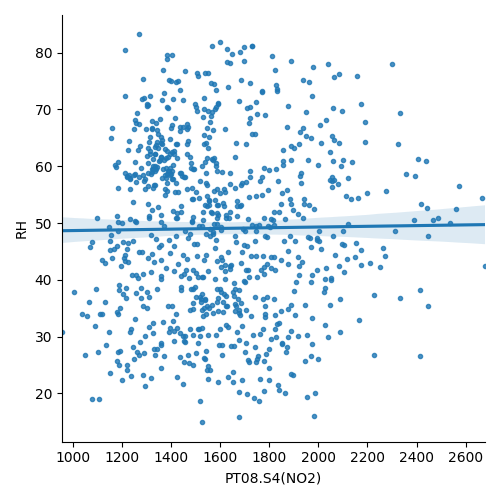
\includegraphics[width=0.3\textwidth]{../images/Figure_9.png}
	\label{线性性}
	}
	\subfigure{
	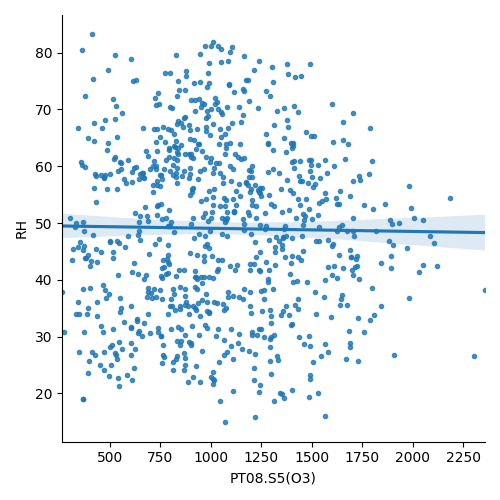
\includegraphics[width=0.3\textwidth]{../images/Figure_10.png}
	\label{线性性}
	}
	\subfigure{
	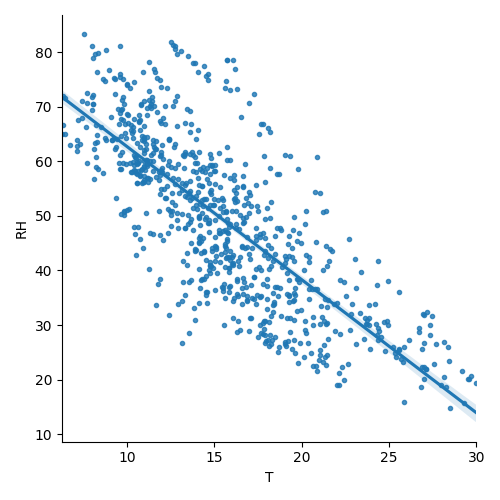
\includegraphics[width=0.3\textwidth]{../images/Figure_11.png}
	\label{线性性}
	}
	\subfigure{
	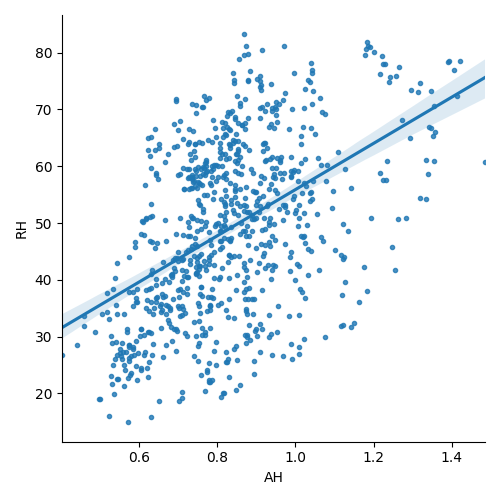
\includegraphics[width=0.3\textwidth]{../images/Figure_13.png}
	\label{线性性}
	}
	\subfigure{
	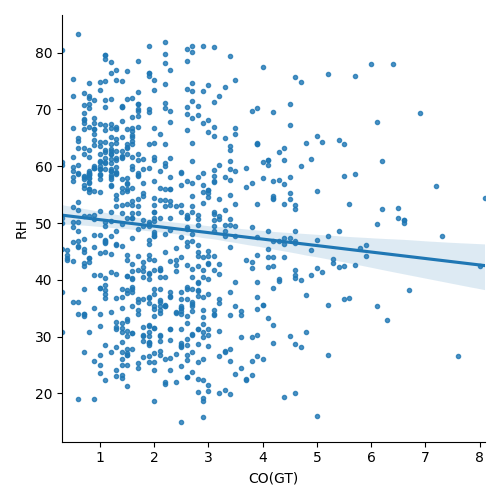
\includegraphics[width=0.3\textwidth]{../images/Figure_19.png}
	\label{线性性}
	}
	\caption{线性性关系}	
\end{figure}
\begin{figure}[H]
	%\centering
	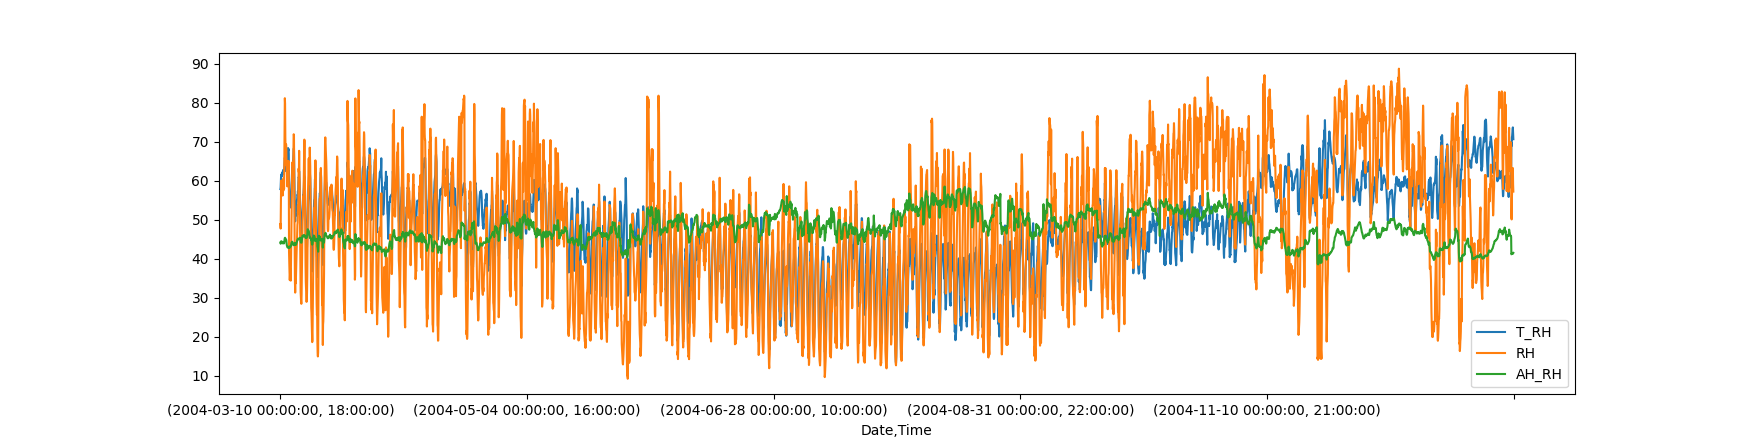
\includegraphics[width=1.2\textwidth]{../images/siganlpa.png}
	\caption{利用单变量回归效果(训练集)}
\end{figure}
\begin{figure}[H]
	%\centering
	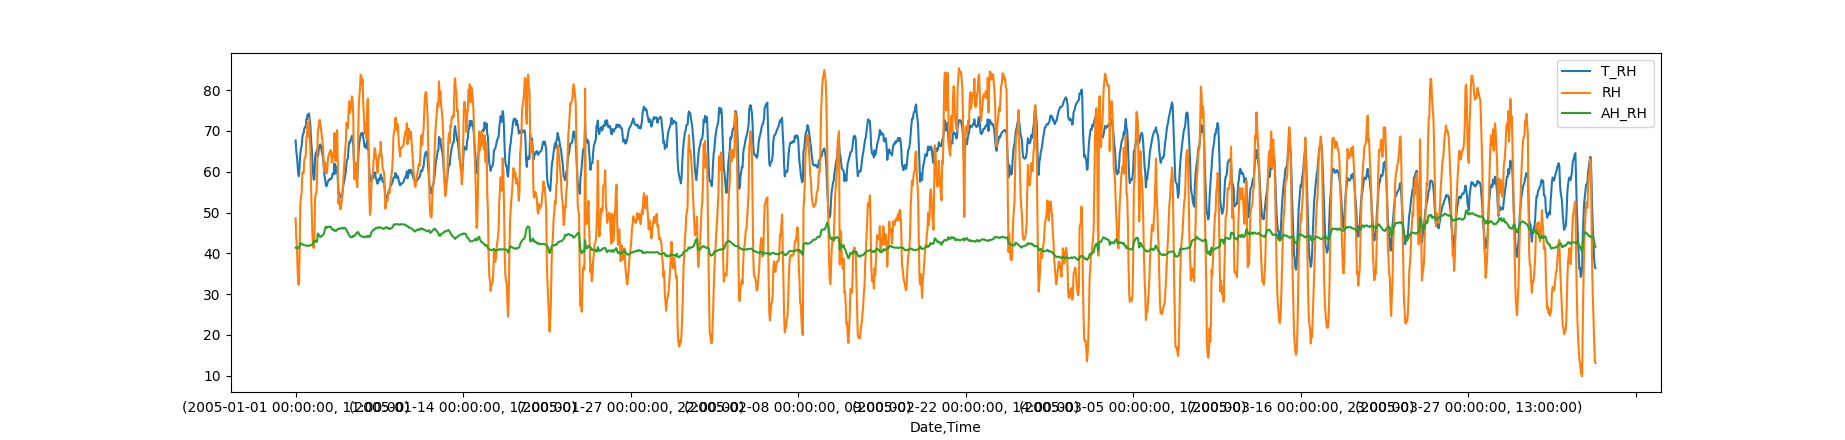
\includegraphics[width=1.2\textwidth]{../images/st.png}
	\caption{利用单变量回归效果(测试集)}
\end{figure}

\subsection{多变量数据之间的线性关系}
直观对比发现,多变量的拟合能力更强,通过其他变量的预测本领更厉害。
\begin{figure}[H]
	%\centering
	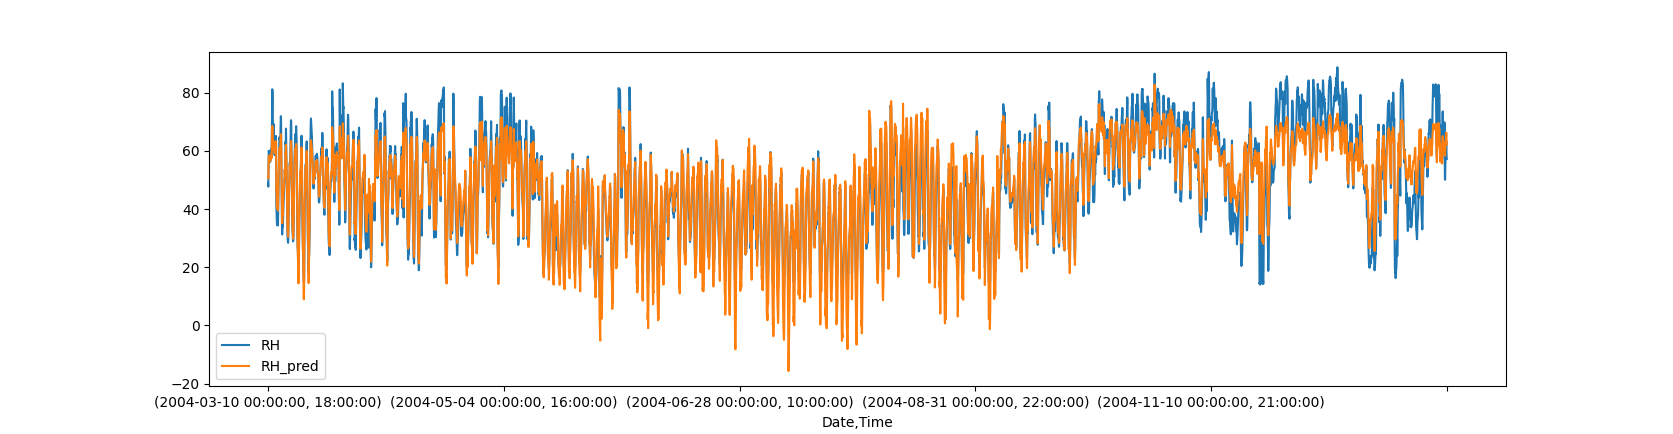
\includegraphics[width=1.2\textwidth]{../images/muti.png}
	\caption{利用多变量回归效果(训练集)}
\end{figure}
\begin{figure}[H]
	%\centering
	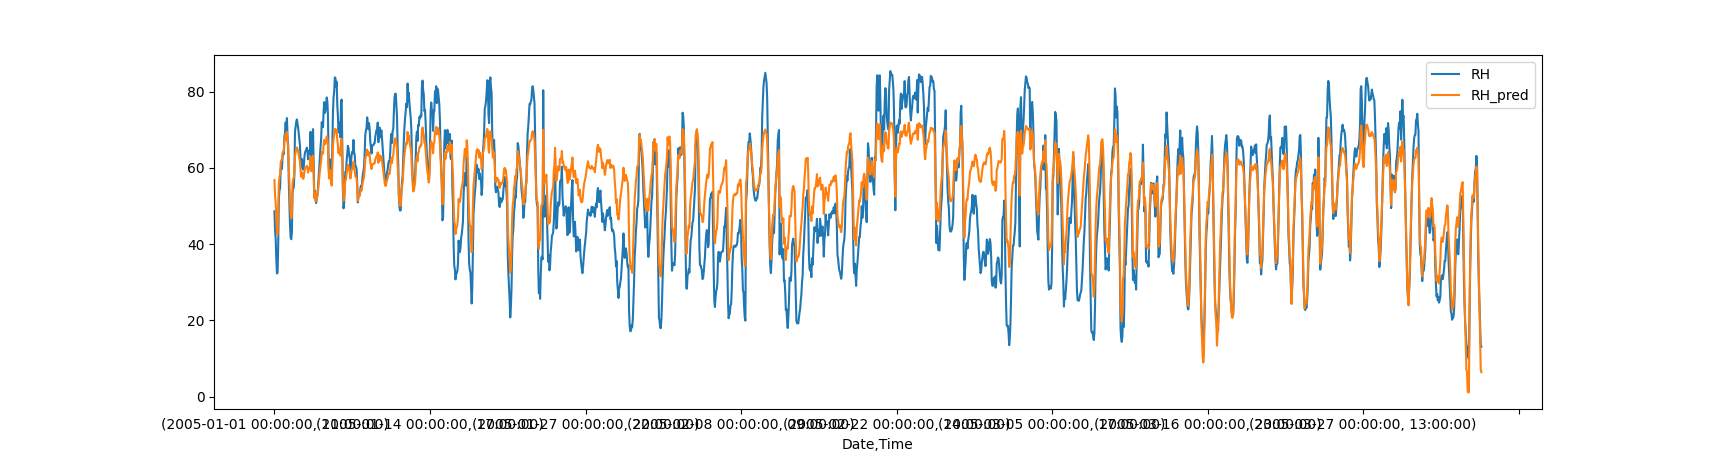
\includegraphics[width=1.2\textwidth]{../images/mx.png}
	\caption{利用多变量回归效果(测试集)}
\end{figure}

\section{多项式回归}
\subsection{算法介绍}
多项式回归是回归分析的一种形式,其中自变量$ x $和因变量$ y $之间的关系被建模为关于$ x $的$ n $次多项式。多项式回归拟合$x$的值与$ y $的相应条件均值之间的非线性关系,表示为$ E(y|x)$,并且已被用于描述非线性现象。虽然多项式回归是拟合数据的非线性模型,但作为统计估计问题,它是线性的。在某种意义上,回归函数$ E(y|x)$ 在从数据估计到的未知参数中是线性的。因此,多项式回归被认为是多元线性回归的特例。\\
多项式回归模型:
\begin{equation}
{\displaystyle y_{i}\,=\,\beta _{0}+\beta _{1}x_{i}+\beta _{2}x_{i}^{2}+\cdots +\beta _{m}x_{i}^{m}+\varepsilon _{i}\ (i=1,2,\dots ,n)}
\end{equation}
可以写成矩阵形式:
\begin{equation}
{\displaystyle {\begin{bmatrix}y_{1}\\y_{2}\\y_{3}\\\vdots \\y_{n}\end{bmatrix}}={\begin{bmatrix}1&x_{1}&x_{1}^{2}&\dots &x_{1}^{m}\\1&x_{2}&x_{2}^{2}&\dots &x_{2}^{m}\\1&x_{3}&x_{3}^{2}&\dots &x_{3}^{m}\\\vdots &\vdots &\vdots &\ddots &\vdots \\1&x_{n}&x_{n}^{2}&\dots &x_{n}^{m}\end{bmatrix}}{\begin{bmatrix}\beta _{0}\\\beta _{1}\\\beta _{2}\\\vdots \\\beta _{m}\end{bmatrix}}+{\begin{bmatrix}\varepsilon _{1}\\\varepsilon _{2}\\\varepsilon _{3}\\\vdots \\\varepsilon _{n}\end{bmatrix}},}
\end{equation}
根据线性回归的知识可以有:
\begin{equation}
{\displaystyle {\widehat {\vec {\beta }}}=(\mathbf {X} ^{\mathsf {T}}\mathbf {X} )^{-1}\;\mathbf {X} ^{\mathsf {T}}{\vec {Y}},\,}
\end{equation}
\subsection{算法实现}
\begin{file}[poly.py]
	\begin{lstlisting}[language=Python]
#! /usr/bin/python
def polyX(X, Y, n=1):
  Keep= []
  for i in range(n+1):
    X_ = X**i
    Keep.append(X_)
  X = np.stack(Keep, axis=1)
  Y = np.array(Y)
  XTXinv=np.linalg.inv(np.matmul(X.transpose(),X))
  XTY = np.matmul(X.transpose(), Y)
  return np.matmul(XTXinv, XTY)
	\end{lstlisting}
\end{file}
\subsection{二阶多项式回归效果}
\begin{figure}[H]
	%\centering
	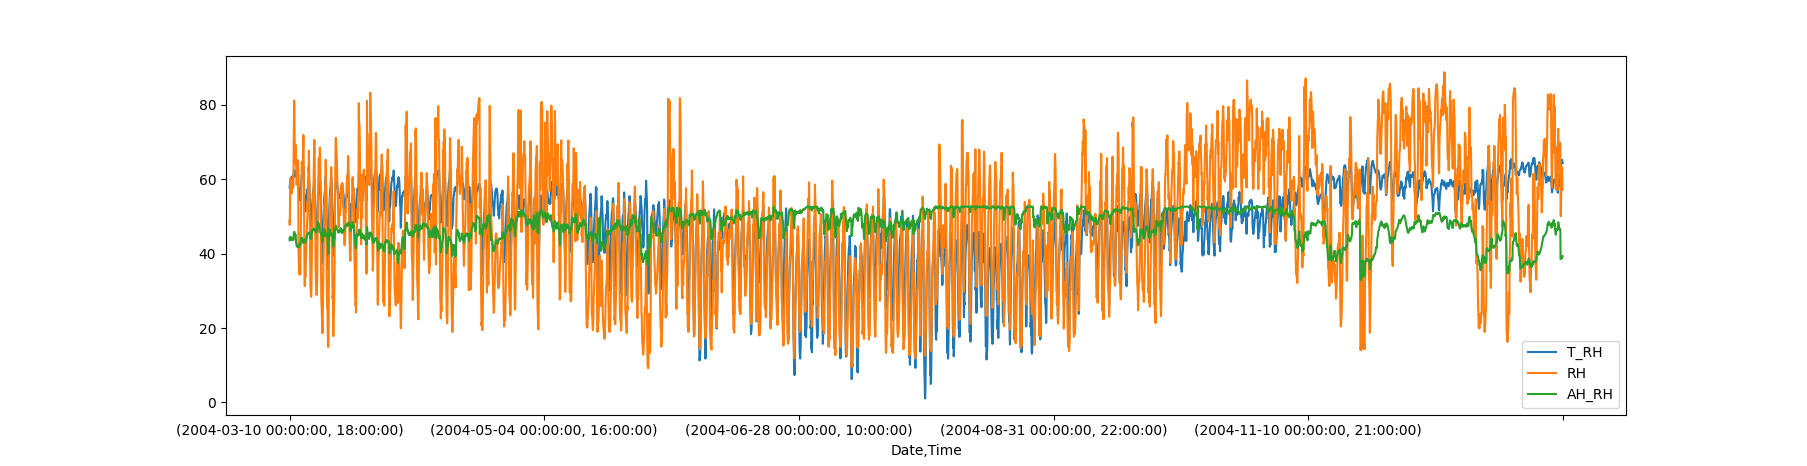
\includegraphics[width=1.2\textwidth]{../images/poly1.png}
	\caption{二阶多项式回归效果(训练集)}
\end{figure}
\begin{figure}[H]
	%\centering
	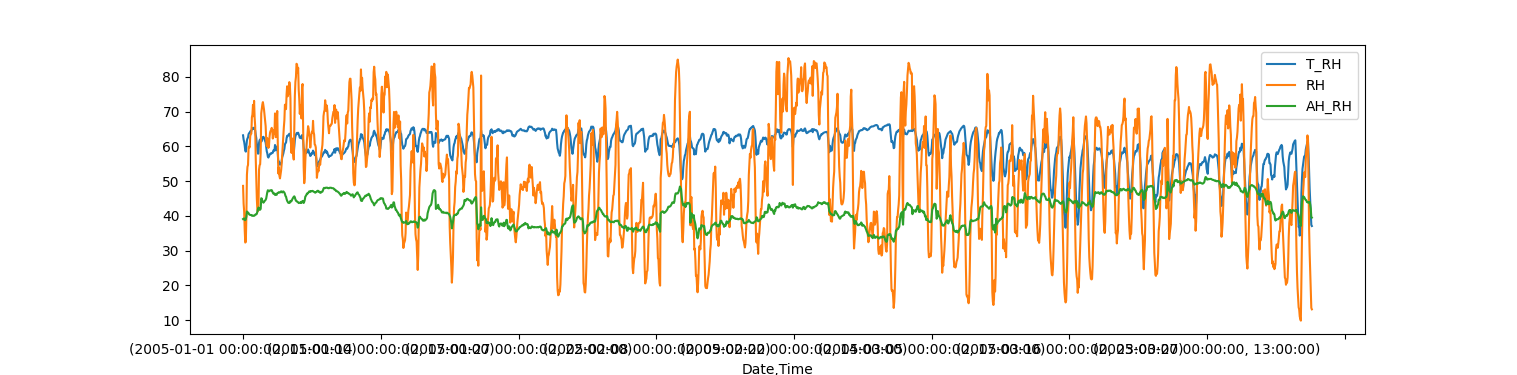
\includegraphics[width=1.2\textwidth]{../images/poly2.png}
	\caption{二阶多项式回归效果(测试集)}
\end{figure}
\subsection{三阶多项式回归效果}
\begin{figure}[H]
	%\centering
	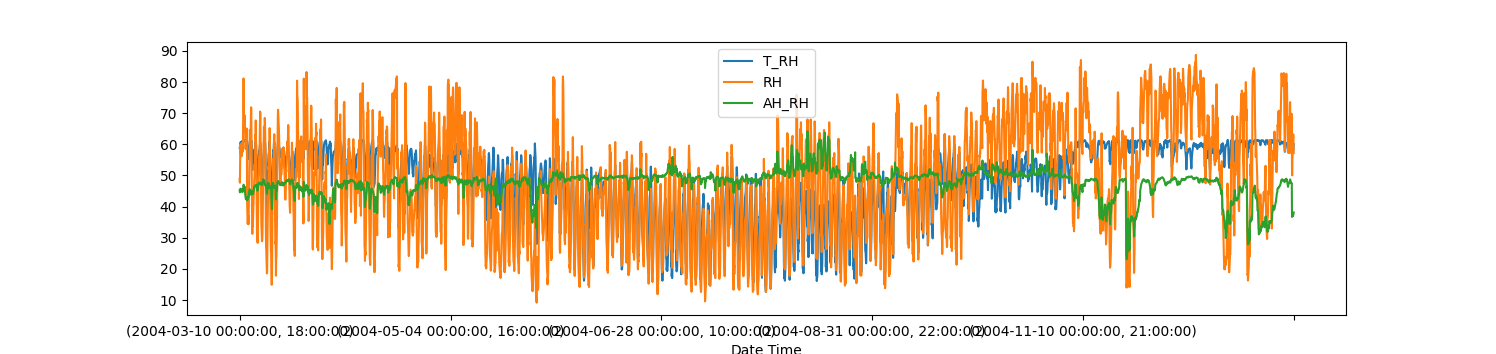
\includegraphics[width=1.2\textwidth]{../images/poly3.png}
	\caption{三阶多项式回归效果(训练集)}
\end{figure}
\begin{figure}[H]
	%\centering
	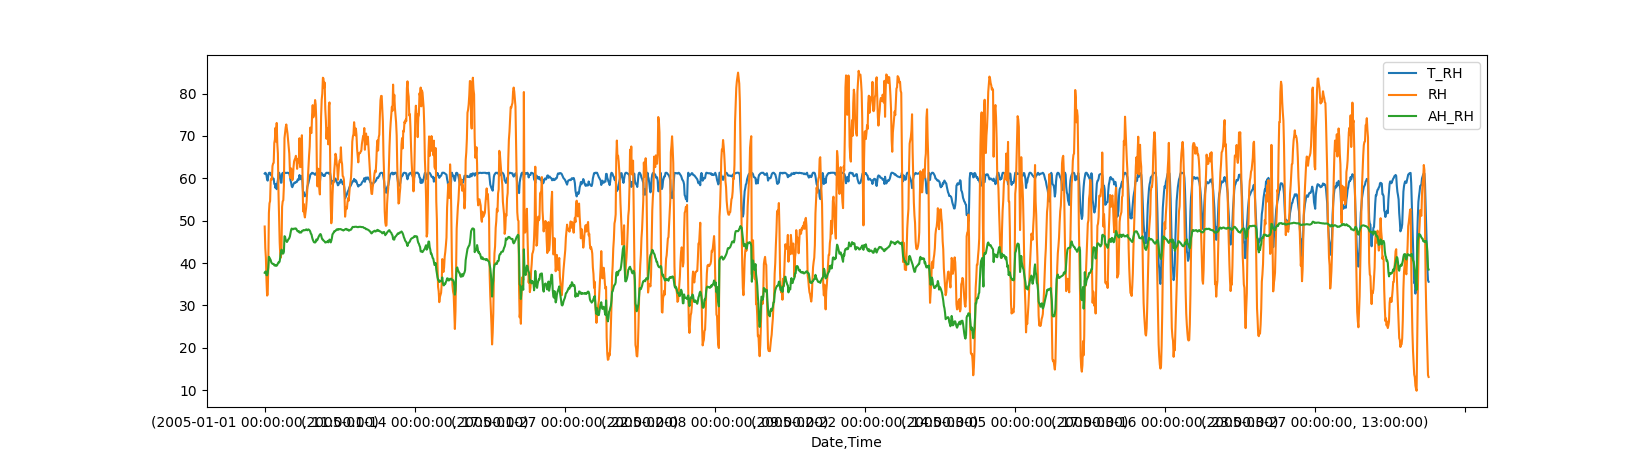
\includegraphics[width=1.2\textwidth]{../images/poly4.png}
	\caption{三阶多项式回归效果(测试集)}
\end{figure}
\subsection{四阶多项式回归效果}
可以看到四阶多项式已经出现了严重的震荡效果,在实际预测上,出现了肉眼可辨识的大幅度偏差
\begin{figure}[H]
	%\centering
	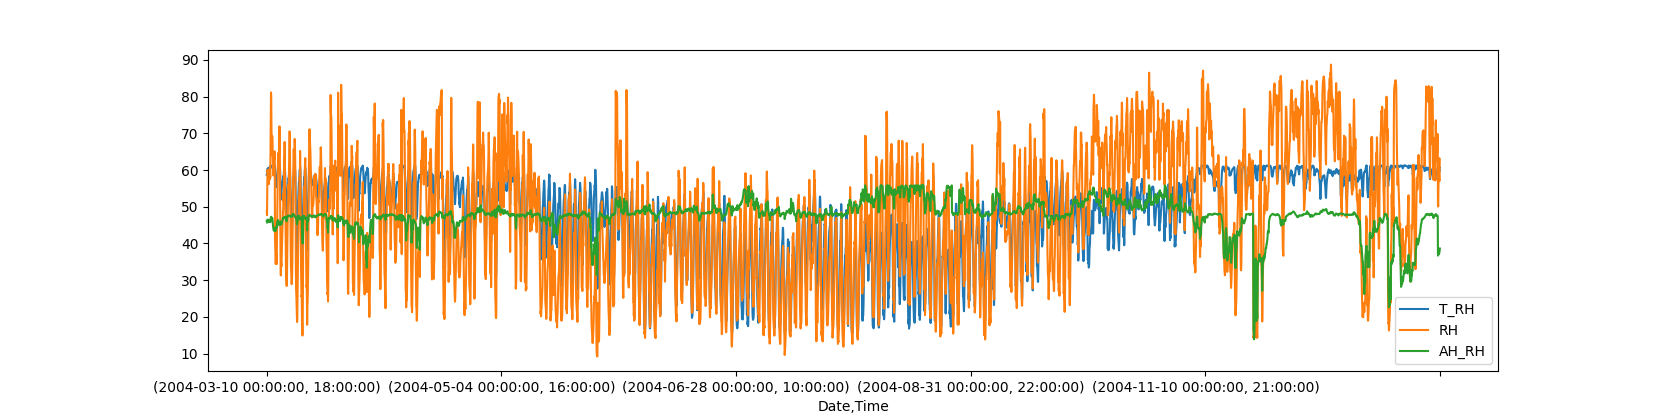
\includegraphics[width=1.2\textwidth]{../images/poly5.png}
	\caption{四阶多项式回归效果(训练集)}
\end{figure}
\begin{figure}[H]
	%\centering
	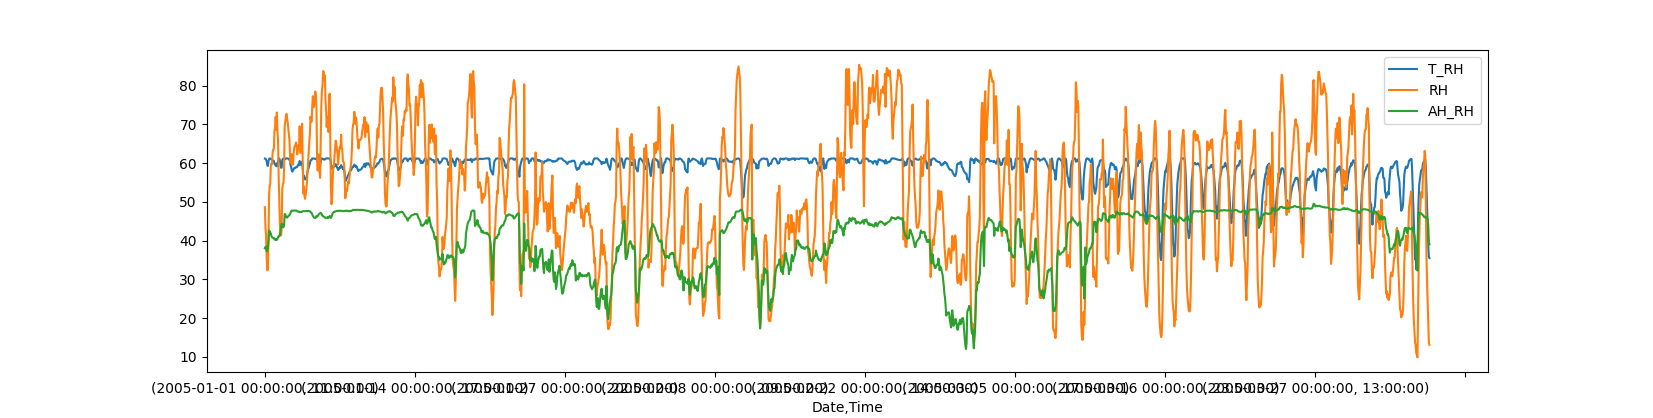
\includegraphics[width=1.2\textwidth]{../images/poly6.png}
	\caption{四阶多项式回归效果(测试集)}
\end{figure}
\subsection{多变量二阶多项式回归效果}
多变量多项式回归的拟合效果以及预测效果都是很不错的,但是次数过高会导致震荡的发生,因此就没有采用过高次幂的多项式多变量回归。
\begin{figure}[H]
	%\centering
	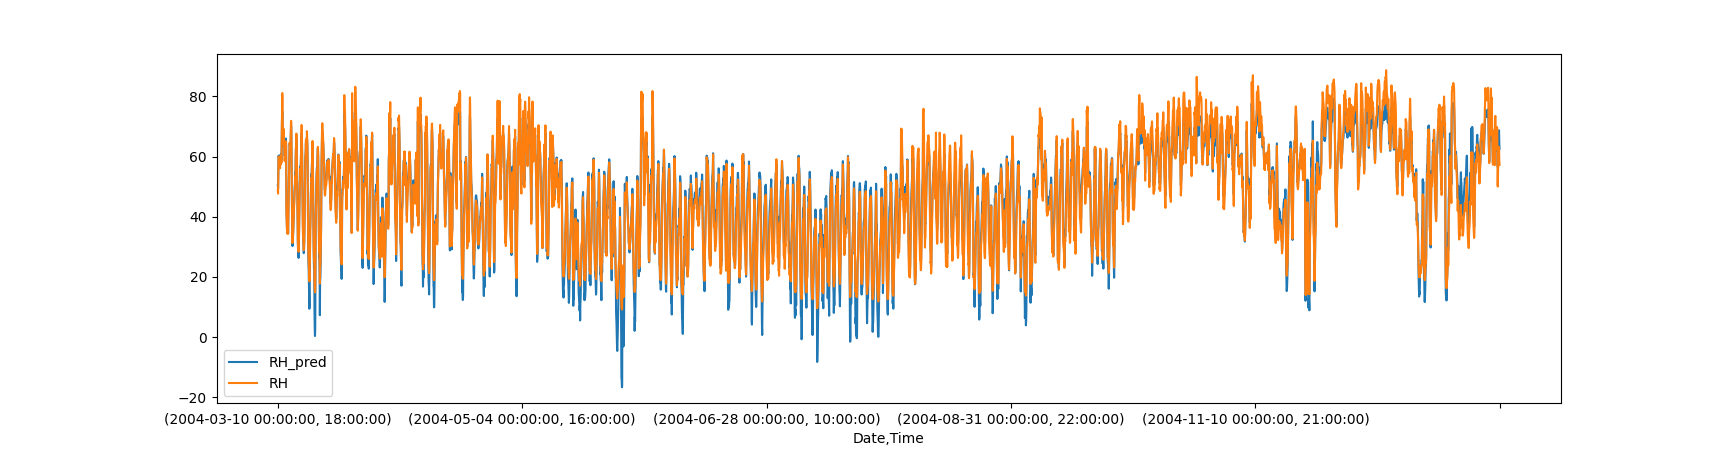
\includegraphics[width=1.2\textwidth]{../images/poly7.png}
	\caption{多变量多项式回归效果(训练集)}
\end{figure}
\begin{figure}[H]
	%\centering
	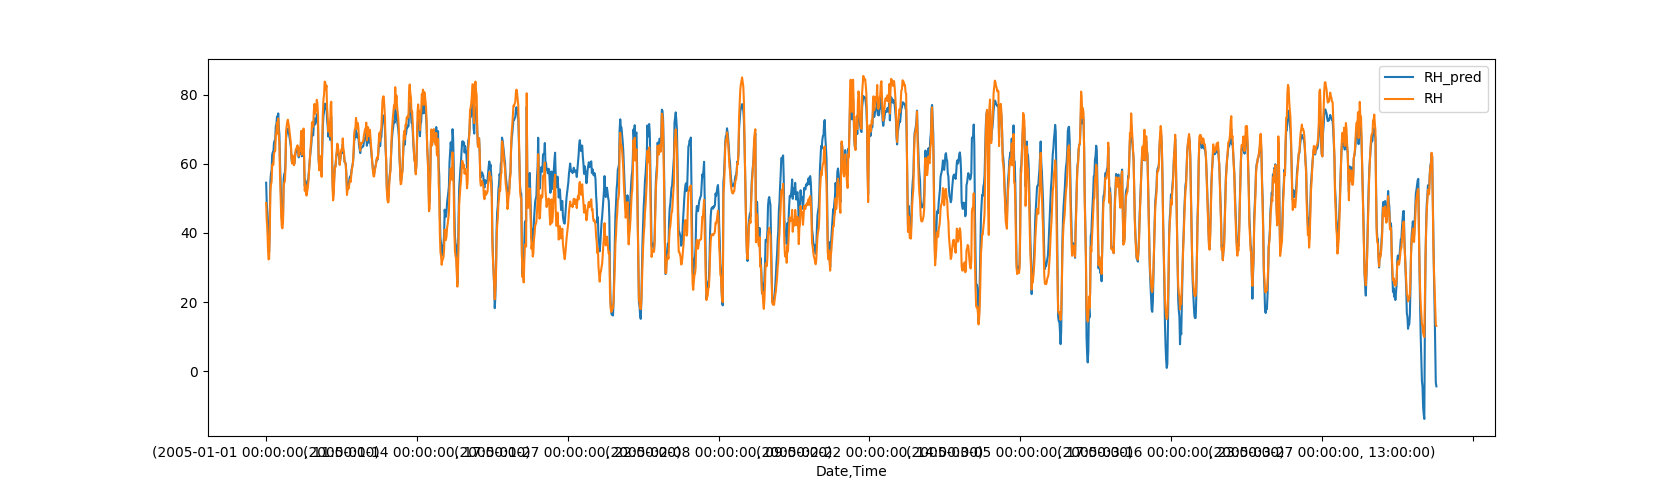
\includegraphics[width=1.2\textwidth]{../images/poly8.png}
	\caption{多变量多项式回归效果(测试集)}
\end{figure}
虽然说阶数越高,拟合本领在局部会越强,这里采用了一个九阶的高阶项,意在说明,震荡会发生,在学习数理方程以及计算方法中,这个现象叫做龙格现象。
\begin{figure}[H]
	%\centering
	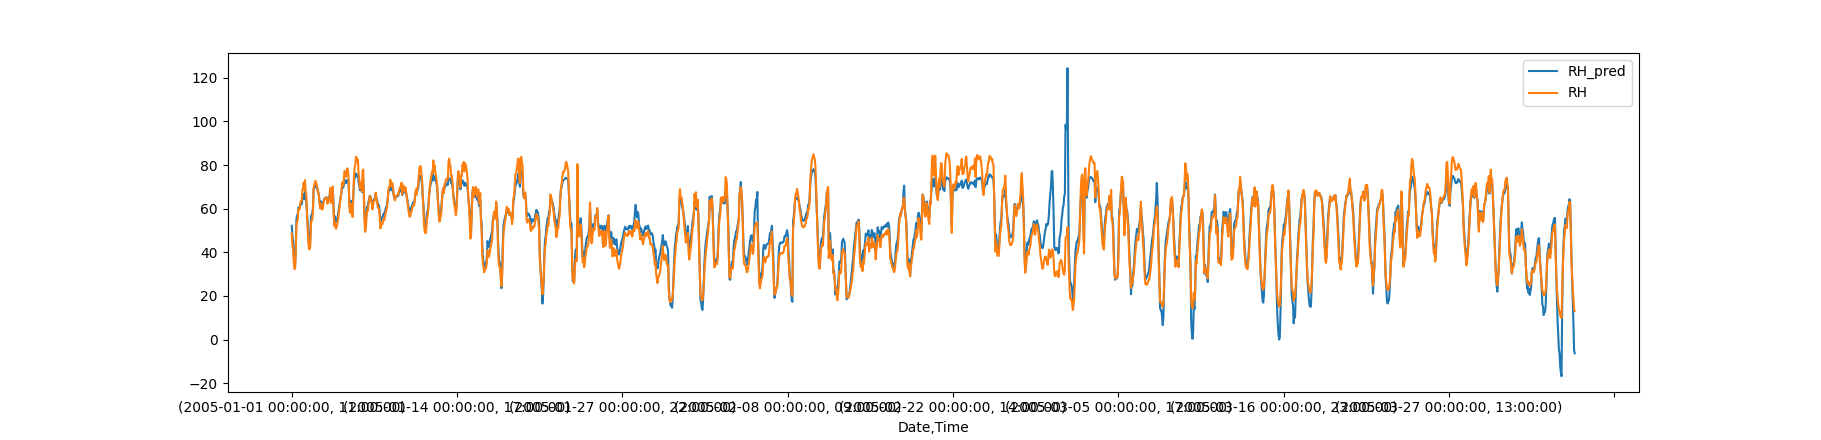
\includegraphics[width=1.2\textwidth]{../images/poly9.png}
	\caption{九阶多变量多项式回归震荡效果}
\end{figure}
\section{岭回归}
\subsection{算法介绍}
岭回归是一种专用于共线性数据分析的有偏估计回归方法,实质上是一种改良的最小二乘估计法,通过放弃最小二乘法的无偏性,以损失部分信息、降低精度为代价获得回归系数更为符合实际、更可靠的回归方法,对病态数据的拟合要强于最小二乘法。

回归分析中常用的最小二乘法是一种无偏估计。对于一个适定问题,$X$通常是列满秩的。当$X$不是列满秩时,或者某些列之间的线性相关性比较大时,$X^TX$的行列式接近于0,即$X^TX$
接近于奇异,上述问题变为一个不适定问题,此时,计算$(X^TX)^{-1}$时误差会很大,传统的最小二乘法缺乏稳定性与可靠性。

为了解决上述问题,我们需要将不适定问题转化为适定问题:我们为上述损失函数加上一个正则化项,变为
\begin{equation}
	Loss = ||X\beta - Y||^2 + ||\alpha I\beta||^2
\end{equation}
于是:
\begin{equation}
		\beta = (X^TX + \alpha I)^{-1} \ X^T Y
\end{equation}
$\alpha$是一个未知变量,可以不断调整找到合适的$\alpha$值。在这个过程中$\beta$在不断地变化,这就是所说的迹岭。
\subsection{算法实现}
下面列出算法逻辑:
\begin{center}
	\begin{minipage}{0.5\linewidth} % Adjust the minipage width to accomodate for the length of algorithm lines
		\begin{algorithm}[H]
			\KwIn{$(X, Y)$, two floating-point matrix}  % Algorithm inputs
			\KwResult{$\beta$, matrix} % Algorithm outputs/results
			\medskip
			
			%\begin{algorithmic}
			\For{$\alpha \in {0.01, 100}$}
			{
				{$\beta_{current} = (X^TX + \alpha I)^{-1} \ X^T Y$} \;
				{$loss_{current} = ||X\beta - Y||^2 + ||\alpha I\beta||^2$} \;
				\If{$loss_{current} < loss_{best}$}
				{
					$loss_{best} = loss_{current}$ \;
					$\beta_{best} = \beta_{current}$
				}
			}
			%\end{algorithmic}
			
			{\bf return} $\beta_{best}$ \;
			\caption{\texttt{岭回归算法}} % Algorithm name
			\label{alg:fastTwoSum}   % optional label to refer to
		\end{algorithm}
	\end{minipage}
\end{center}
\begin{file}[ridge.py]
	\begin{lstlisting}[language=Python]
	#! /usr/bin/python
def ridgeX(X, Y):
  X = np.array(X)
  Y = np.array(Y)
  X = np.stack([X, np.ones(X.shape[0])], 1)
  best_loss = MAX
  Beta_best = np.eye(1)
  loss = []
  for i in np.arange(0.01,20000,0.4) :
    XTX = np.matmul(X.transpose(), X)
    XTY = np.matmul(X.transpose(), Y)
    XTX_I = XTX+i*np.eye(XTX.shape[0])
    Beta_c = np.matmul(np.linalg.inv(XTX_I),
             XTY)
  Y_pred = np.matmul(X,
       Beta_c[..., None]).squeeze(1)
  loss_c = np.sum((Y-Y_pred)**2) + \
       np.sum((i*np.matmul(np.eye(XTX.shape[0]),
  Beta_c))**2)
  loss.append(loss_c)
  if loss_c < best_loss:
    best_loss = loss_c
    Beta_best = Beta_c
  return Beta_best
	\end{lstlisting}
\end{file}
\subsection{岭回归误差曲线}
从全局看,岭迹分析可用来估计在某一具体问题中最小二乘估计是否适用,把回归系数的岭迹都绘制在一张图上,如果这些曲线比较稳定,如图18所示,利用最小二乘估计会有一定的把握,这个问题下由于选用的$X$比较合适,可以达到无偏的效果,因此岭回归不适合这个问题,但是依旧可以做一下。
\begin{figure}[H]
	\centering
	\subfigure{	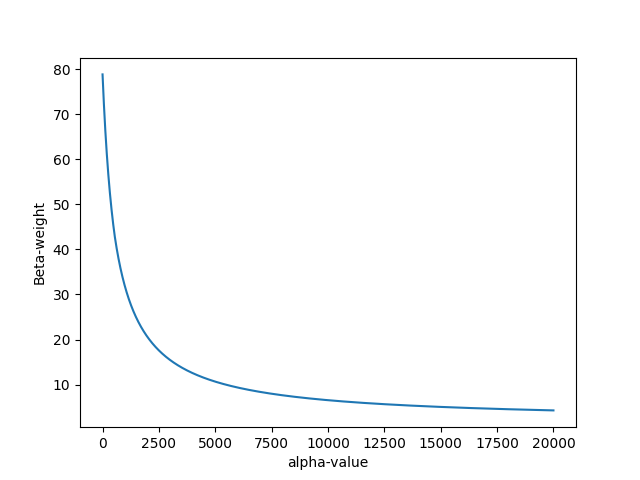
\includegraphics[width=0.3\textwidth]{../images/rig3.png}}
	\subfigure{	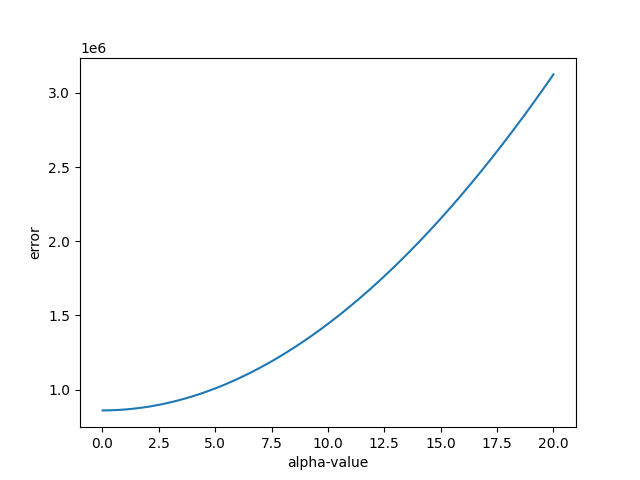
\includegraphics[width=0.3\textwidth]{../images/rig4.png}}
	\caption{岭迹图(左), 误差曲线(右)}
\end{figure}
\subsection{岭回归效果}
\begin{figure}[H]
	%\centering
	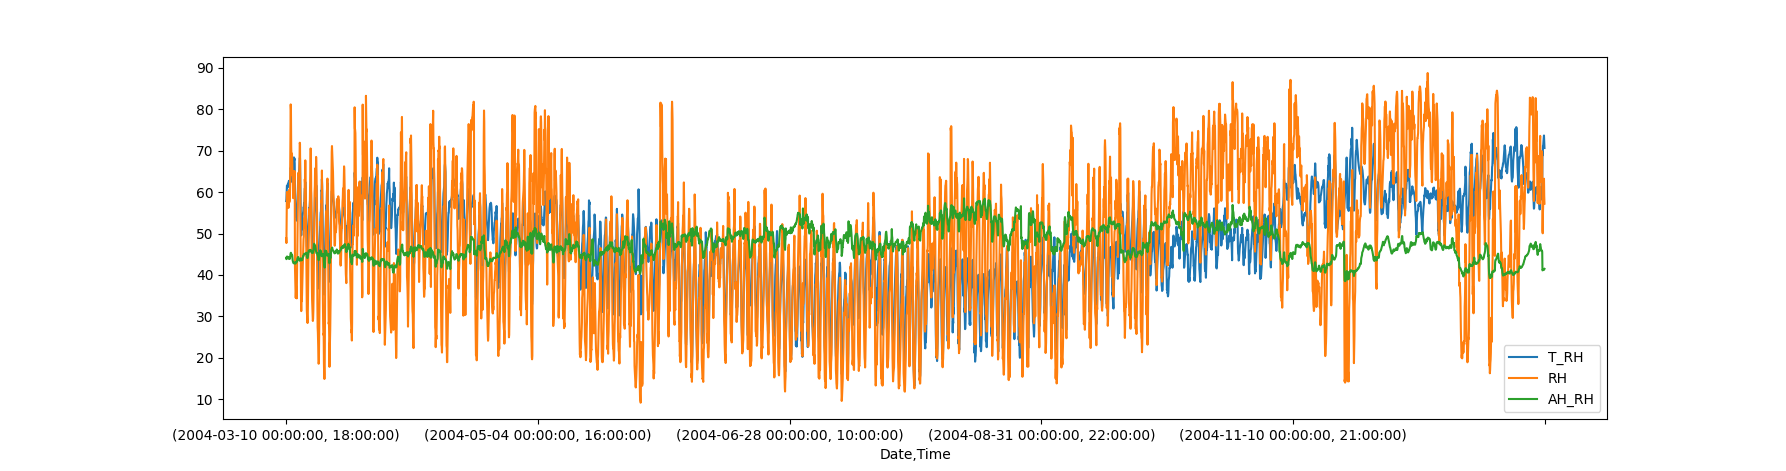
\includegraphics[width=1.2\textwidth]{../images/rig1.png}
	\caption{岭回归效果(训练集)}
\end{figure}
\begin{figure}[H]
	%\centering
	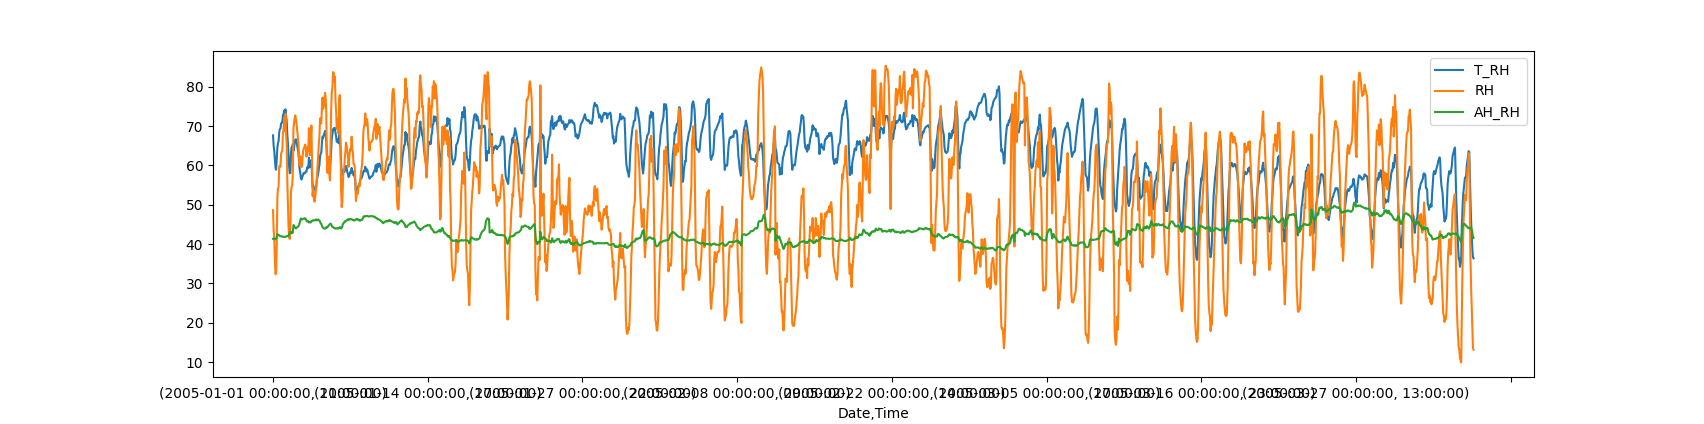
\includegraphics[width=1.2\textwidth]{../images/rig2.png}
	\caption{岭回归效果(测试集)}
\end{figure}


\section{支持向量回归 SVR}
\subsection{算法介绍}
支持向量分类的方法可以扩展来解决回归问题。此方法称为支持向量回归。通过支持向量分类生成的模型仅取决于训练数据的子集(支持向量),因为构建模型的成本函数并不关心超出裕度(最大化间隔)的训练点。类似地,由支持向量回归产生的模型仅取决于训练数据的子集,因为成本函数会忽略预测接近其目标的样本。
\begin{figure}[H]
	%\centering
	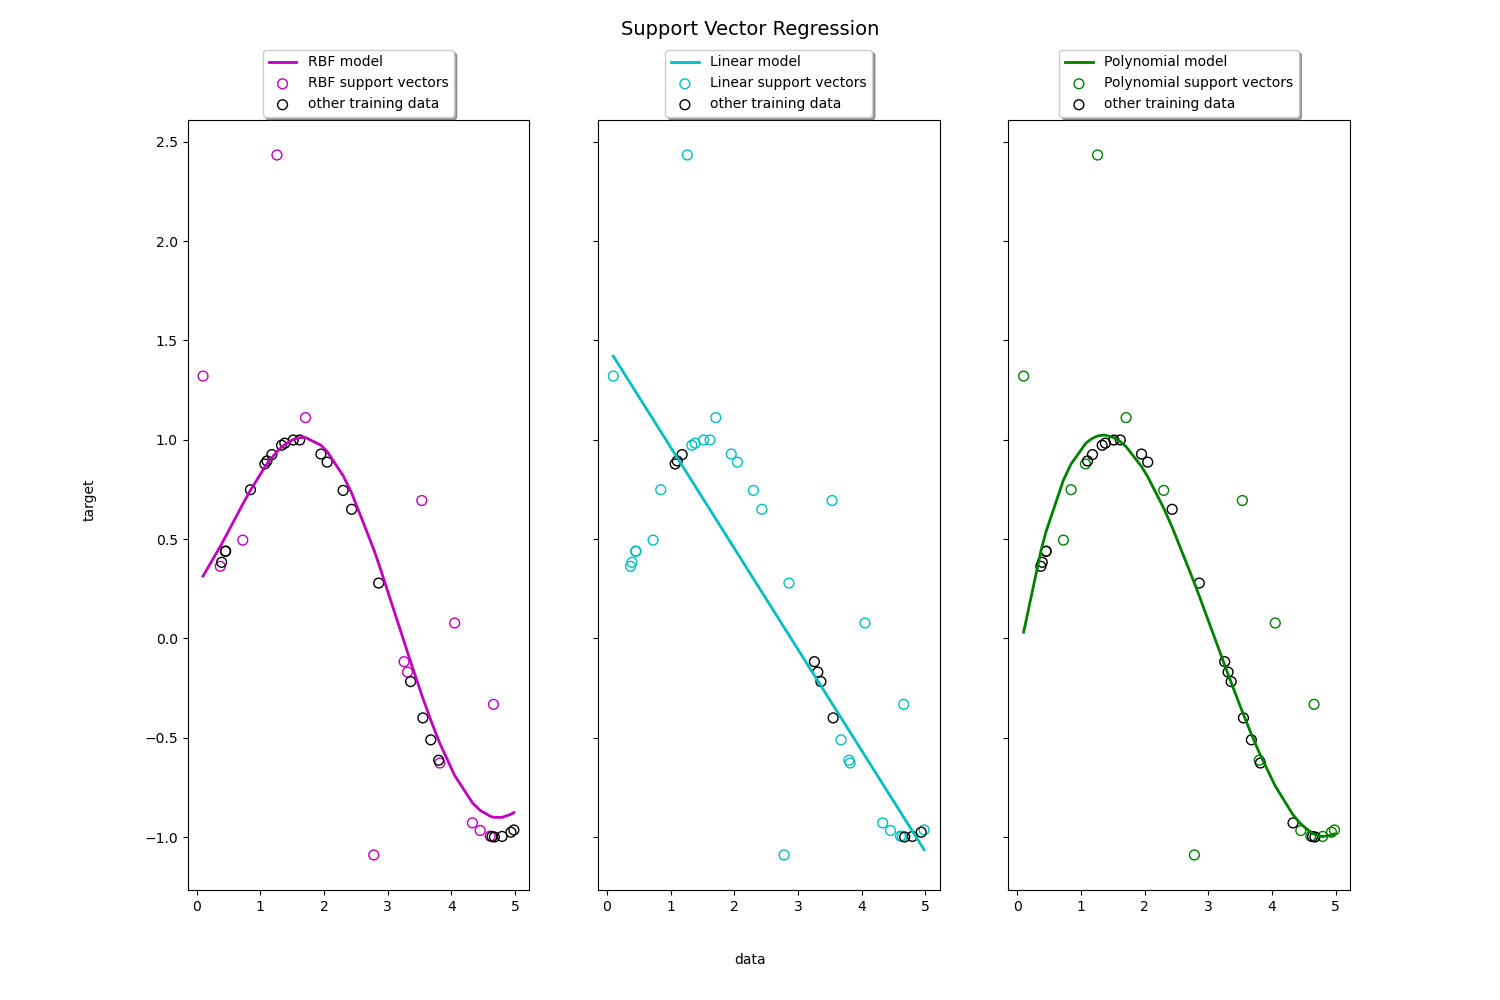
\includegraphics[width=1\textwidth]{../images/svr0.png}
	\caption{支持向量回归算法示意}
\end{figure}
\subsection{支持向量分类}
给定训练向量$x_i \in \mathbb{R}^p$,对于一个二分类问题,有分类目标$y \in \{1, -1\}^n$,分类目标可以简述为,寻找参数$w$以及$b$,使得预测$\text{sign} (w^T\phi(x) + b)$对于大多数情况是正确的。


描述软间隔SVC问题($\zeta_i$固定为0,没有惩罚项的情况为硬间隔SVC问题)为:
\begin{equation}
\min_ {w, b, \zeta} \frac{1}{2} w^T w + C \sum_{i=1}^{n} \zeta_i\\
\end{equation}
\begin{equation}
	\begin{split}\textrm {st.  \ \ \  } & y_i (w^T \phi (x_i) + b) \geq 1 - \zeta_i,\\
	& \zeta_i \geq 0, i=1, ..., n\end{split}
\end{equation}


支持向量机的核心思想是最大化间隔,也就是最小化$||W||^2 = W^T W$(这里有一定的推导过程,整体在于归一化思想就把最大化转为了最小化),软间隔的思想是允许一定量的误差可以发生。

上式的对偶问题为:
\begin{equation}
 \min_{\alpha} \frac{1}{2} \alpha^T Q \alpha - e^T \alpha\\ 
\end{equation}
\begin{equation}
	\begin{split}
	\textrm {st. \ \ \ \ \  } & y^T \alpha = 0\\
	& 0 \leq \alpha_i \leq C, i=1, ..., n\end{split}
\end{equation}
为了应对可能出现的非线性可分情况,需要对输入向量$x_i \in \mathbb{R}^p$做高维映射,通常采用的方法为核函数,改写决策方程:
\begin{equation}
	\sum_{i\in SV} y_i \alpha_i K(x_i, x) + b
\end{equation}


\subsection{支持向量回归}
给定训练向量$x_i \in \mathbb{R}^p$,以及预测目标$y \in \mathbb{R}^n$,SVR解决的问题可以描述为下:
 \begin{align}\begin{aligned} \min_ {w, b, \zeta, \zeta^*} \frac{1}{2} w^T w + C \sum_{i=1}^{n} (\zeta_i + \zeta_i^*)\\\end{aligned}\end{align} 
\begin{equation}
	\begin{split}\textrm {st.\ \ \ \     } & y_i - w^T \phi (x_i) - b \leq \varepsilon + \zeta_i,\\
	& w^T \phi (x_i) + b - y_i \leq \varepsilon + \zeta_i^*,\\
	& \zeta_i, \zeta_i^* \geq 0, i=1, ..., n\end{split}
\end{equation}
其中$\zeta_i$与$\zeta^{*}_i$为惩罚项,类似于上述的软间隔方案,可以提供一定的误差空间,两个惩罚项各自代表这上下与回归预测误差空间。

上式的对偶问题为:
\begin{equation}
	 \min_{\alpha, \alpha^*} \frac{1}{2} (\alpha - \alpha^*)^T Q (\alpha - \alpha^*) + \varepsilon e^T (\alpha + \alpha^*) - y^T (\alpha - \alpha^*)\\
\end{equation}
\begin{equation}
	\begin{split}
	\textrm {st.  \ \ \ \ \  \ \ \ \ \ \ \ } & e^T (\alpha - \alpha^*) = 0\\
	& 0 \leq \alpha_i, \alpha_i^* \leq C, i=1, ..., n\end{split}
\end{equation}
\subsection{算法流程}
\begin{info} % Information block
	这部分采用sklearn机器学习库中的内容进行SVR实验,具体详见相关代码
\end{info}

\begin{file}[svr.py]
\begin{lstlisting}[language=Python]
#! /usr/bin/python
def svr(kernel="linear", T="M", test=False):
	from sklearn.svm import SVR
	engine = SVR(kernel)
\end{lstlisting}
\end{file}

\subsection{SVR 效果}
\begin{figure}[H]
	%\centering
	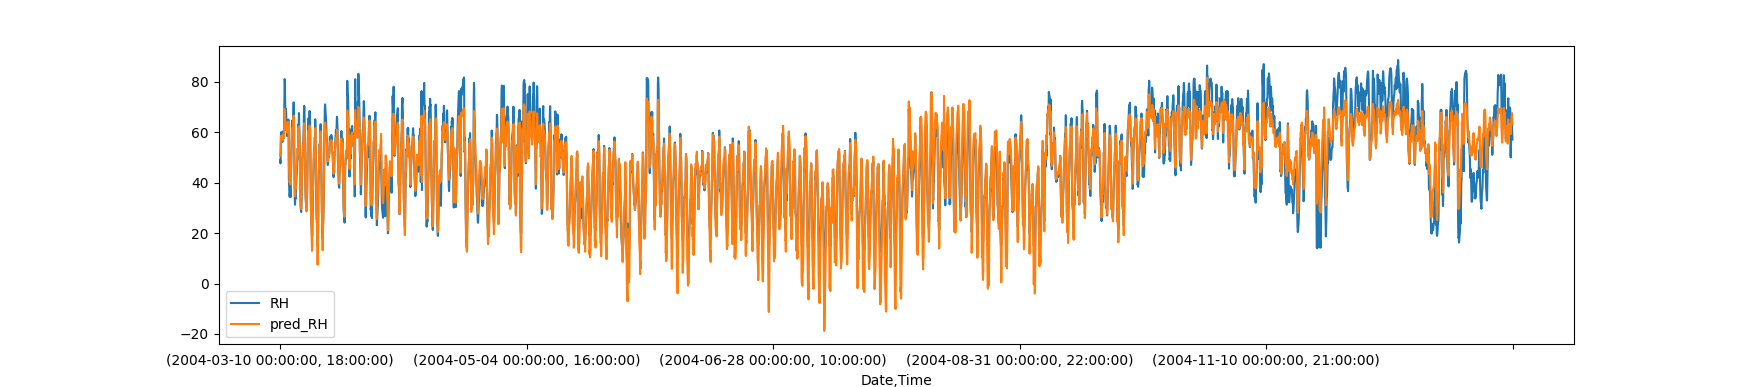
\includegraphics[width=1.2\textwidth]{../images/svr1.png}
	\caption{多变量线性支持向量回归效果(训练集)}
\end{figure}
\begin{figure}[H]
	%\centering
	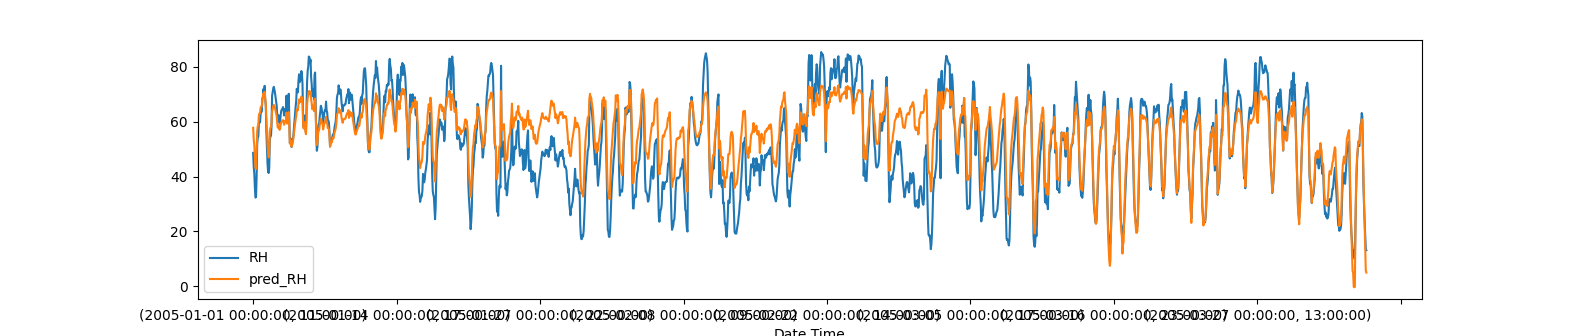
\includegraphics[width=1.2\textwidth]{../images/svr2.png}
	\caption{多变量线性支持向量回归效果(测试集)}
\end{figure}

\begin{figure}[H]
	%\centering
	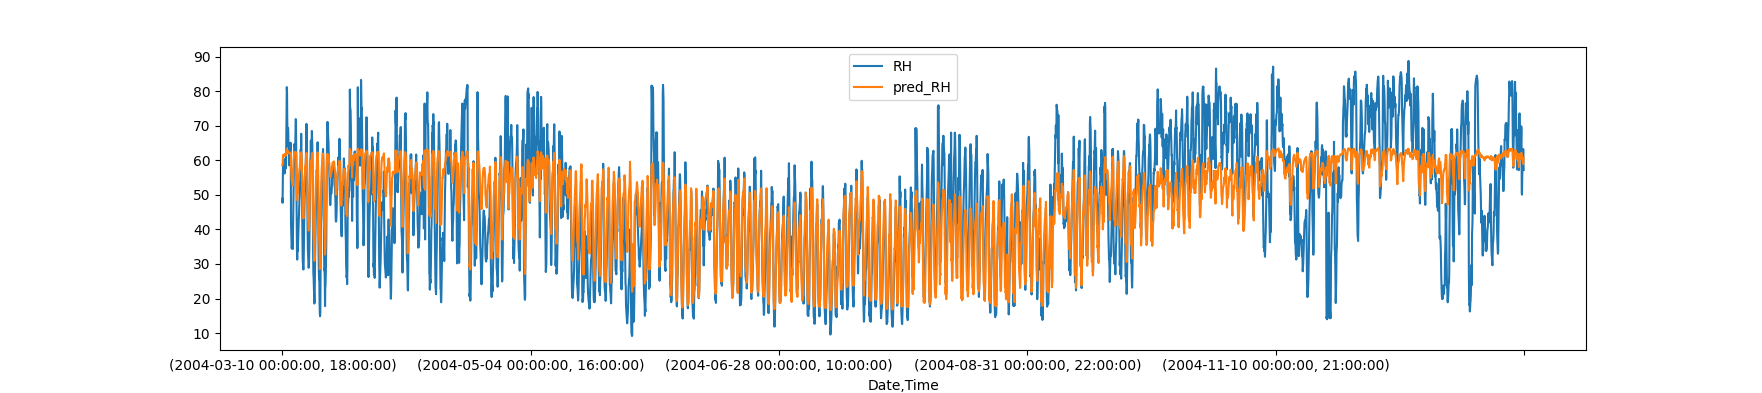
\includegraphics[width=1.2\textwidth]{../images/svr3.png}
	\caption{多变量RBF支持向量回归效果(训练集)}
\end{figure}
\begin{figure}[H]
	%\centering
	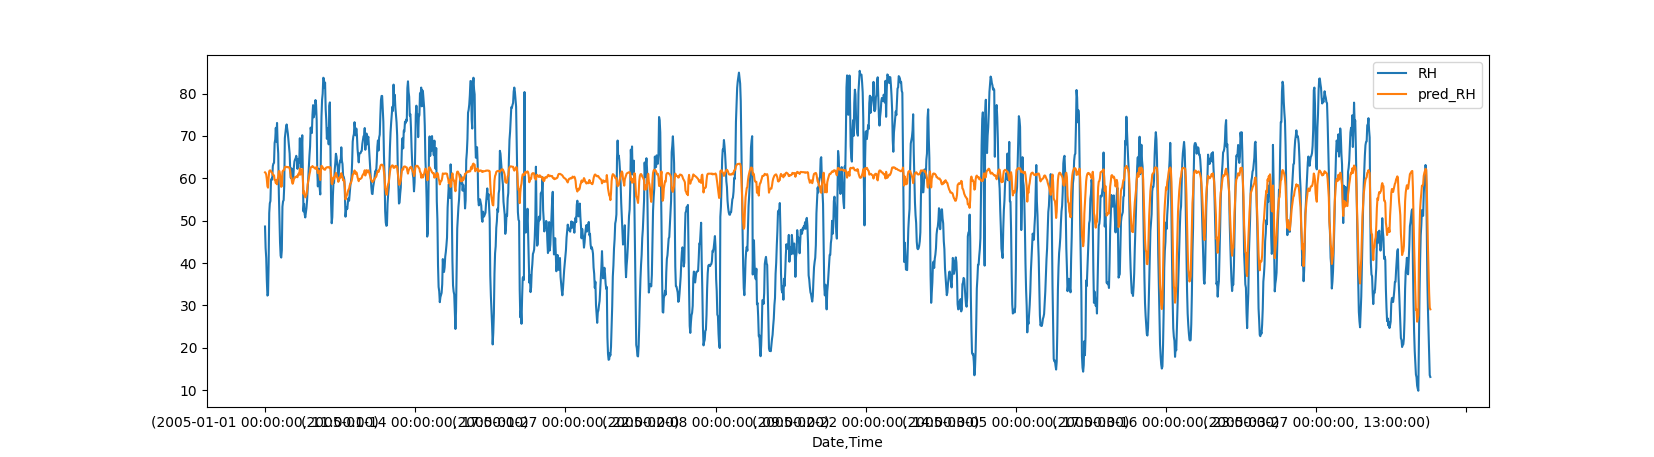
\includegraphics[width=1.2\textwidth]{../images/svr4.png}
	\caption{多变量RBF支持向量回归效果(测试集)}
\end{figure}

\begin{figure}[H]
	%\centering
	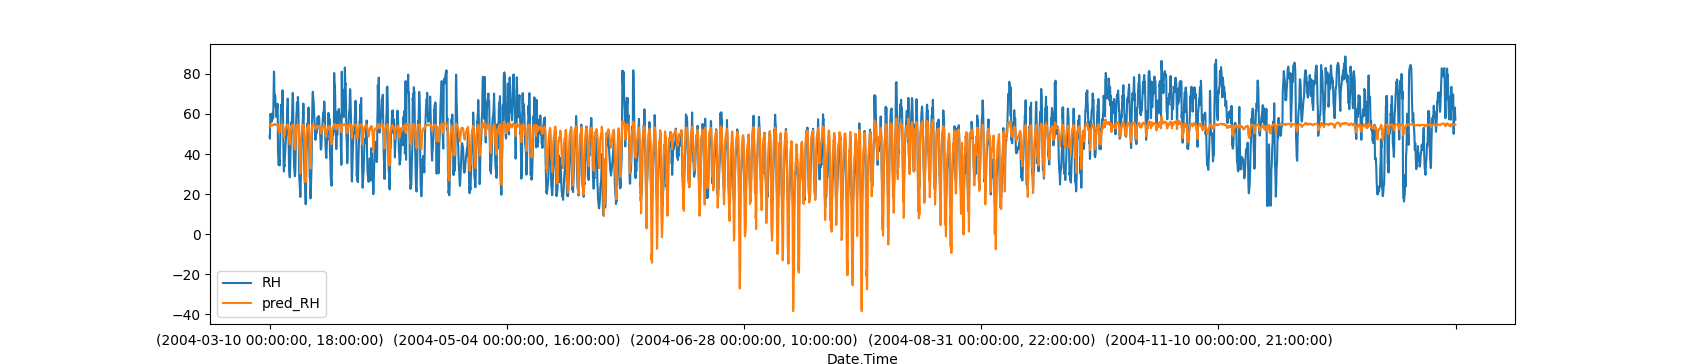
\includegraphics[width=1.2\textwidth]{../images/svr5.png}
	\caption{多变量多项式支持向量回归效果(训练集)}
\end{figure}
\begin{figure}[H]
	%\centering
	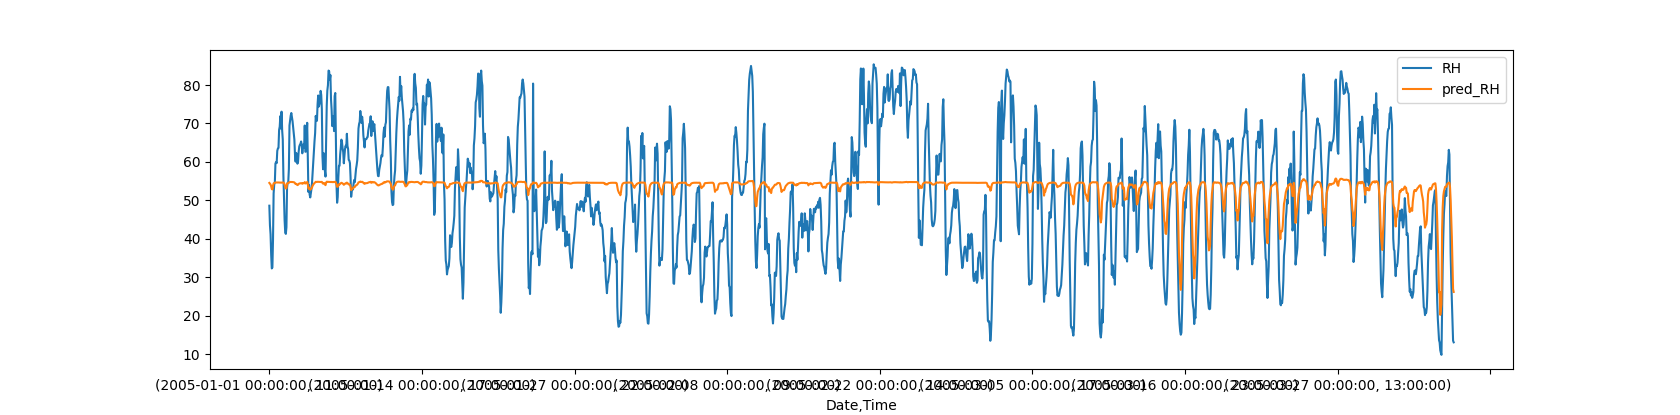
\includegraphics[width=1.2\textwidth]{../images/svr6.png}
	\caption{多变量多项式支持向量回归效果(测试集)}
\end{figure}
\section{总结}
\subsection{算法性能对比}
\subparagraph{误差曲线对比} 下面对上述所有多变量方法进行算法的误差曲线评估,单变量一定效果是不如多变量的,在上文中已经多次验证,因此下文就对多变量效果进行分析。
\begin{figure}[H]
	%\centering
	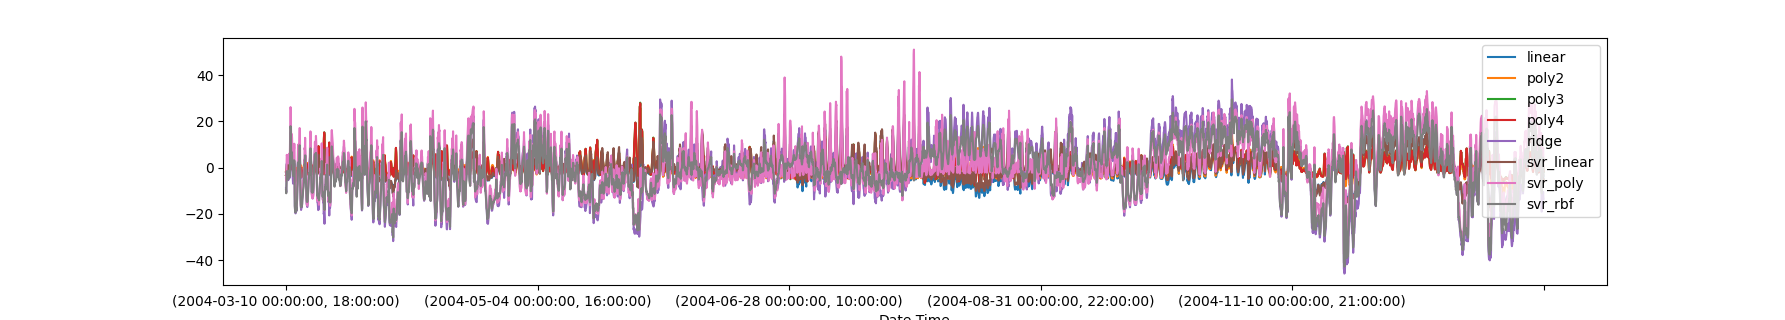
\includegraphics[width=1.2\textwidth]{../images/e1.png}
	\caption{多变量误差曲线(训练集)}
\end{figure}
\begin{figure}[H]
	%\centering
	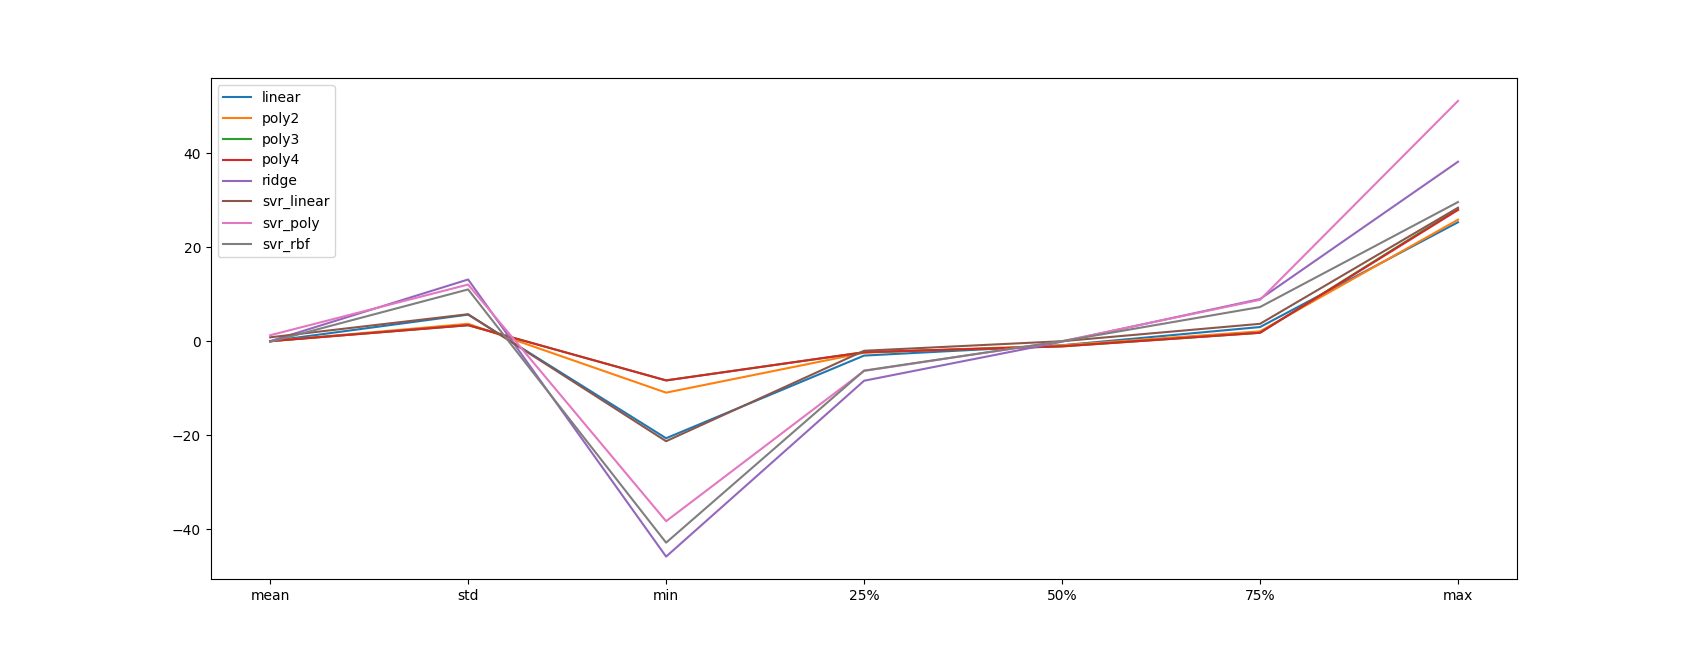
\includegraphics[width=1.2\textwidth]{../images/e3.png}
	\caption{多变量误差基本属性}
\end{figure}
\begin{figure}[H]
	%\centering
	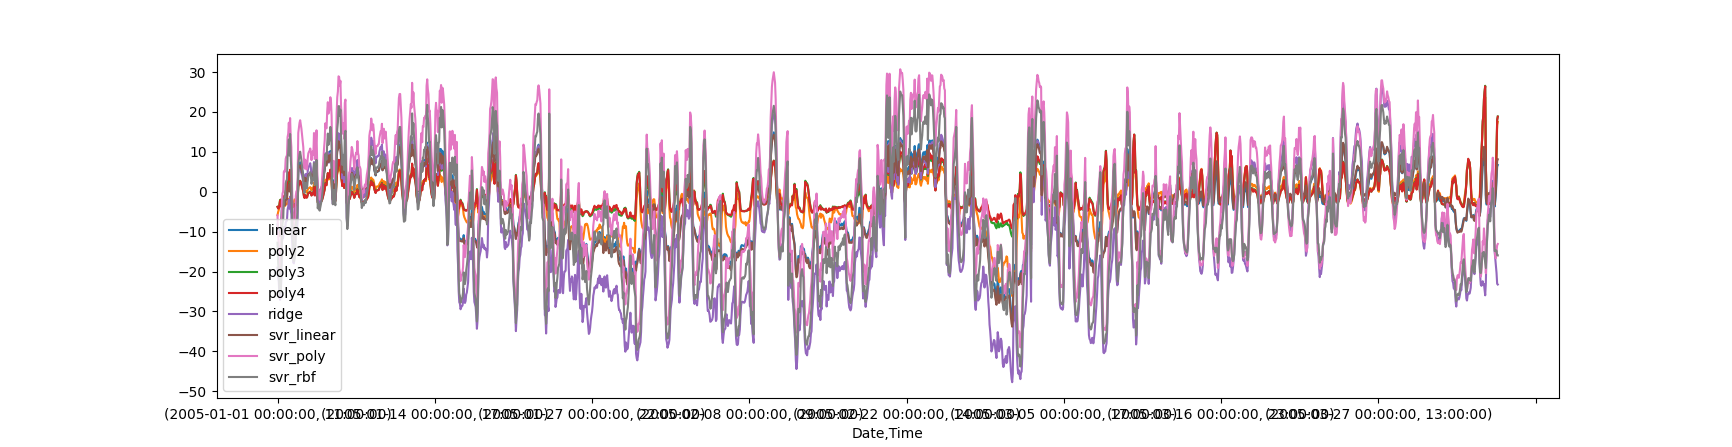
\includegraphics[width=1.2\textwidth]{../images/e2.png}
	\caption{多变量误差曲线(训练集)}
\end{figure}
\begin{figure}[H]
	%\centering
	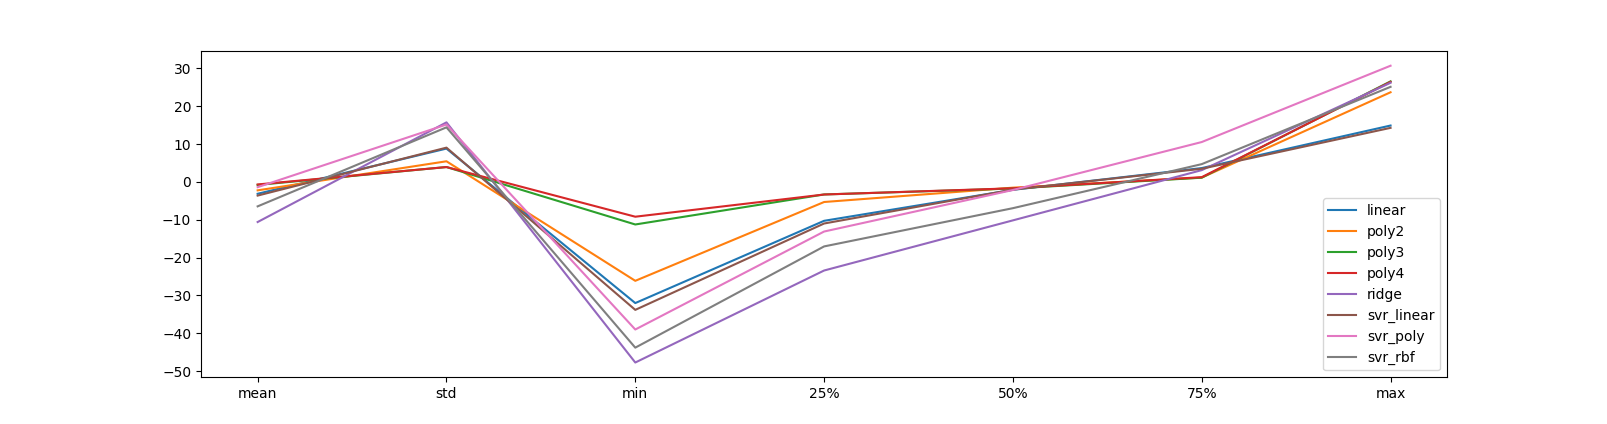
\includegraphics[width=1.2\textwidth]{../images/e4.png}
	\caption{多变量误差基本属性}
\end{figure}
可以看到,多项式型多变量回归模型是效果最好的,同时岭回归和线性模型以及线性支持向量回归属性很相近,但是他们的出发原理是不同的,岭回归由于这个问题下的特殊性,自然是和线性模型很近似,如果我设置的岭回归参数足够小,那么应该理论上会是一个线性模型。
\subparagraph{计算时间对比}
\begin{figure}[H]
	%\centering
	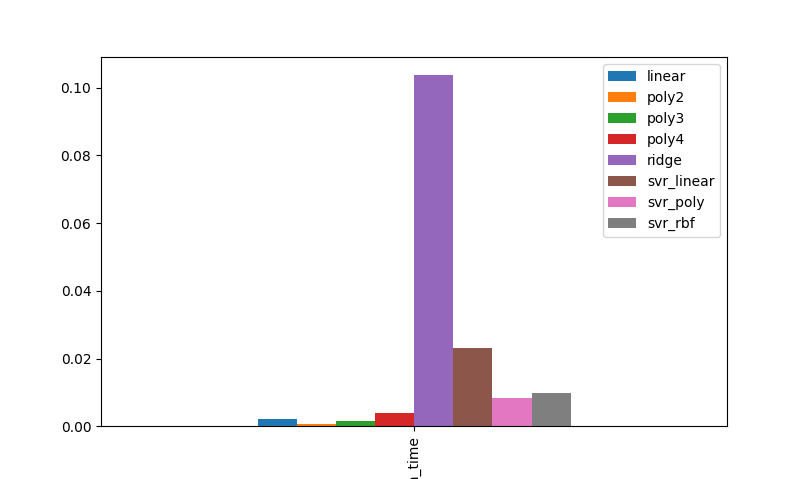
\includegraphics[width=0.8\textwidth]{../images/e5.png}
	\caption{算法时间对比}
\end{figure}
二阶效率比线性还快,后面查资料发现,是因为二阶模型会使得矩阵变为范德猛矩阵,可以加速计算,同样在支持向量回归的对比上也验证了这点,因为SVR我是采用的调包的方式。而岭回归花费时间较长是因为参数的选择,我采用遍历的方式,比较耗费时间。
\subsection{总结与感想}
在商务智能大作业中,我选择去探究一下回归分析的内容,学习包括线性回归,多项式回归,多变量多项式回归,以及岭回归,了解到岭回归是在矩阵不满秩,变量有强相关性的基础下诞生的,当然,在我选定的题目条件下,这个问题不适用于岭回归的技巧,通过岭迹图可以看到稳定的变化曲线,本次最重要的是,以前都是调包实现回归分析,这次通过自己手写这几个方案,感受到回归算法不一样的味道,最小二乘法在本次实验中起到了非常重要的作用,其实对于最小二乘还有其他的拓展形式,为了达到在线学习的目的,可以改为递推最小二乘,以及考虑方差的加权最小二乘,和用在数据处理过程中的移动最小二乘。以及最后去学习支持向量回归的内容,以前接触过支持向量机,所以学习的难度不是很大,主要是思维的转变,支持向量机一般被用在分类问题上,在回归问题上还是第一次遇到,思路的确很不错。



%----------------------------------------------------------------------------------------
%	PROBLEM 2
%----------------------------------------------------------------------------------------

\section{Implementation}

本次实验所有代码采用python3.6完成,运行环境为ubuntu20.04, 安装依赖方法为:

% Command-line "screenshot"
\begin{commandline}
	\begin{verbatim}
		$ pip3  -r install ./requirements.txt
		$ python3 ./linear.py  #线性回归
		$ python3 ./poly.py    #多项式回归
		$ python3 ./ridge.py   #岭回归
		$ python3 ./svr.py     #支持向量回归
		$ python3 ./time.py    #对比算法时间

	\end{verbatim}
\end{commandline}


% Warning text, with a custom title
\begin{warn}[Notice:]
  代码同步放到 https://github.com/WANGSSSSSSS/regression-learning 仓库。
  具体计算方法,详见各个文件代码。
\end{warn}

%----------------------------------------------------------------------------------------

\end{document}
